%==== Document Setup (usthesis)======================================
\documentclass[report,                       %... Document type
               12pt,oneside,openany,a4paper, %... Layout
               report, a5block,          	%... A5 type block
               afrikaans, english,            %... Afrikaans default language
               ]{usthesis}
               
%==== Language setup ================================================
\usepackage[latin1]{inputenc}%................... Recognizes �, �, etc
\usepackage{babel}%.............................. Language setup

%==== Math setup ====================================================
%\usepackage{amsmath}%............................ Advanced
% math (before fonts) 
%\usepackage{amssymb}%............................ AMS
% Symbol fonts

%==== Font setup (default is Computer Modern) =======================
 \usepackage[T1]{fontenc}%........................ Type 1 fonts
 \usepackage{textcomp}%........................... Additional text character
 \usepackage{bm}%................................. Bold math symbols (after fonts)
 
 %==== Ref's, Bib's and Nomencl ======================================
 \usepackage{usnomencl}%.......................... List of symbols (in usthesis pack)
 \usepackage{usbib}%.............................. Bibliography    (in usthesis pack)
    \bibliographystyle{usmeg-a}
    \renewcommand\bibfont{\small}

    %% For usmeg-a, the bib is a list of references. If you
    %% are using usmeg-n comment out the following lines
    \addto{\captionsafrikaans}{\renewcommand{\bibname}{Lys van Verwysings}}
    \addto{\captionsenglish}{\renewcommand{\bibname}{List of References}}
    
    %==== Graphics and Color ============================================
\usepackage{graphicx}%........................... Graphicx loaded in usthesis
\usepackage{color}%.............................. Color setup

%==== Additional USthesis packages ==================================

\usepackage{ussummary}%.......................... Mech Eng summary page (in usthesis pack)

%==== Local Defs ====================================================
\makeatletter

\usepackage{epstopdf}
\usepackage{url}
%\usepackage{pdfpages}
%
% Please insert user defined commands here
% and NOT in the document itself!
%

\makeatother
%==== Title Page ====================================================

\title{Development of a Cashless Vending Machine}

\author{JC\ Lock}
       {JC Lock \\16016548}

\subject{Mechatronic Project 488}
        {Mechatronic Project 488}

\ReportDescript{Final Report}

\address{Department of Mechanical and Mechatronic Engineering,\\
         Stellenbosch University,\\
         Private Bag X1, Matieland 7602.}

\studyleader{Prof. G-J van Rooyen}

\setdate{10}{2013}

\begin{document}

\frontmatter
%========================================================

\TitlePage
\CopyrightPage
\chapter{Declaration}

I, the undersigned, hereby declare that the work contained within this report is my own, original work.\par
\vspace{1.5cm}

\noindent%
\parbox{.5\textwidth}{%
  Signature:\quad\dotfill\par
  \hfill JC\ Lock\hspace{1.8cm}\null}\vspace{1cm}
\newline

\vspace{1.5cm}
\noindent%
\parbox{.5\textwidth}{%
  Date:\quad\dotfill\par}

\chapter{Acknowledgements}

I would like to thank my project supervisor, Prof. G-J van Rooyen, for his
support throughout this project and J.P. Meijers for his help with some of the
electronic design aspects of this project.
\newline
\newline
Lastly I would like to thank my parents, Koos and Elzahn Lock, my brother and
all my family and friends for their continued support and guidance. 



%*** Summary Heading ************************************************

\begin{Summary}{Mechatronic Project 488: Summary}

   \noindent
   \begin{tabular}{@{}ll@{}}
      \textsf{Student:}  &  JC\ Lock\\
      \textsf{Co-worker:} & N/A
   \end{tabular}

%*** The Summary table **********************************************
\begin{SumTable}
 \hline%=============================================================
 \SumHead{Title of Project}\\
 \hline%=============================================================
 Development of a Cashless Vending Machine.
 \\

 \hline%=============================================================
 \SumHead{Objectives}\\
 \hline%=============================================================
 Program and make a model vending machine which accepts payments made via a cellphone.
 \\

 \hline%=============================================================
 \SumHead{Which aspects of the project are new/unique?}\\
 \hline%=============================================================
 The easy use of simple cellphone technologies most students currently have built into in their
 cellphones, such as NFC and QR Codes.
 \\
   
 \hline%=============================================================
 \SumHead{What are the findings?}\\
 \hline%=============================================================
 A working test model was built which accepts faux money paid with either QR Codes or NFC. All
 the necessary security measures, i.e. encryption and challenge codes, were added as well as a
 central web server that tracks user transactions.
 \\

 \hline%=============================================================
 \SumHead{What value do the results have?}\\
 \hline%=============================================================
 The results show that the machine is working reliably. Some improvements can be made, but the
 overall machine is working as expected.
 \\

 \hline%=============================================================
 \SumHead{If more than one student is involved, what is each one's contribution?}\\
 \hline%=============================================================
 Only one student was involved in this project.
 \\

 \hline%=============================================================
 \SumHead{Which aspects of the project will carry on after completion?}\\
 \hline%=============================================================
 This project has been successfully completed and will therefore not continue.
 \\

 \hline%=============================================================
 \SumHead{What are the expected advantages of continuation?}\\
 \hline%=============================================================
 N/A
 \\

 \hline%=============================================================
 \SumHead{What arrangements have been made to expedite continuation?}\\
 \hline%=============================================================
 N/A
 \\

 \hline%=============================================================
\end{SumTable}

%*** Signatures *****************************************************

\vspace{1.5cm}
\SumSignatures

\end{Summary}

\endinput

%*** THE ABSTRACT PAGE ************************************

\begin{abstract}
   
\end{abstract}

\endinput

\tableofcontents
\listoffigures
\listoftables
\chapter{Nomenclature}

\begin{Nomencl}
 \NomGroup{Acronyms}
   \item[AWS]\dotfill Amazon Web Services
   \item[BJT]\dotfill Bipolar Junction Transistor
   \item[EC2]\dotfill Elastic Compute Cloud
   \item[EMF]\dotfill Electromotive Force
   \item[GPIO]\dotfill General Purpose Input Output
   \item[HTTP]\dotfill Hypertext Transfer Protocol
   \item[HTML]\dotfill Hypertext Markup Language
   \item[i$^2$c]\dotfill Inter-Integrated Circuit
   \item[LLCP]\dotfill Logical Link Control Protocol
   \item[NDEF]\dotfill NFC Data Exchange Format
   \item[NFC]\dotfill Near Field Communication
   \item[OS]\dotfill Operating System
   \item[QR Code]\dotfill Quick Response Code
   \item[RFID]\dotfill Radio Frequency Identification
   \item[RSA]\dotfill Ron Rivest, Adi Shamir and Leonard Adleman
   \item[SNEP]\dotfill Simple NDEF Exchange Protocol
   \item[SPI]\dotfill Serial Peripheral Interface
   \item[SU]\dotfill Stellenbosch University
   \item[USSD]\dotfill Unstructured Supplementary Service Data
   \item[UART]\dotfill Universal Asynchronous Receiver Transmitter
   \item[ZXing]\dotfill Zebra Crossing
 \NomGroup{Variables}
   \item[I]\UnitLine{Current}{A}
   \item[P]\UnitLine{Power}{W}
   \item[V]\UnitLine{Voltage}{V}
   \item[R]\UnitLine{Resistance}{\Omega}
   \item[$\omega$]\UnitLine {Angular Velocity}{rad/sec}
 \NomGroup{Variable Subscripts}
   \item[$b$]\dotfill Base
   \item[$p$]\dotfill Raspberry Pi
   \item[$r$]\dotfill Relay				%Maak spasie issue reg
   \item[$o$]\dotfill Supply Voltage
   \item[$e$]\dotfill Back-EMF
   \NomGroup{Constants}
   \item[$\beta$]\dotfill Transistor Current Amplification  
   \item[k$_e$]\dotfill Back-EMF Constant
\end{Nomencl}

\endinput


\mainmatter
%=========================================================

%\numberwithin{equation}{section}%(from amsmath)
%\numberwithin{figure}{section}  %
%\numberwithin{table}{section}   %

\chapter{Introduction}
\label{chap:1}

\section{Problem Statement}

The Vending Machines (VMs) currently used at Stellenbosch University (SU) exclusively
make use of cash transactions. These VM systems are currently the
de facto standard throughout the world, but they do have one drawback:
they require a hard cash transaction to take place. In a world moving away from
cash transactions and towards online payments, e-transactions and mobile
payments, this may become a problem to potential customers. With that in mind, a need has
been identified at SU for a VM that accepts cashless transactions.

\section{Existing Solutions}

Currently there are cashless payment solutions being used by the general public.
These include debit and credit cards, Radio Field Identification (RFID) cards,
Unstructured Supplementary Service Data (USSD) based systems and, more recently, Near
Field Communication (NFC) payments. These alternatives are further discussed in this
section.

\subsection{Credit and Debit Cards}

A familiar and widely-used alternative to cash payments are the debit and
credit cards most modern adults possess. This is especially
true in developed countries with mature and reliable financial institutions.

The advantages these cards hold over the other cashless options are
that they are easy to obtain and that they have become very
reliable and simple to use. A disadvantage is that debit and credit systems may become
costly and complicated to implement. This is very true for the simple system developed in
this project.

\subsection{Radio Field Identification}

RFID is a technology which was first patented in 1983
[\cite{patent:nfc-patent}]. Since then, the technology has grown and matured into a very
reliable identification and payment platform. Examples of where this is used are the
payments made to new parking meters with a contactless card.

The advantage of this technology is its great convenience: a customer only needs
to tap the card against a receiver and it is not required that a password be
entered.

However, this leads to some security concerns. For example, if the card gets stolen
or cloned, the thief can use the money on the card for his own benefit.
Fortunately, these cards most commonly work with pre-paid money.
Therefore, provided that there was not too much money loaded onto the card, the
theft victim will not suffer a financial loss greater than if cash were stolen. 

\subsection{Unstructured Supplementary Service Data}

USSD is a communication standard used by cellphones to exchange data with a
service provider's servers. If the service provider allows it, USSD may be used by a customer to make financial transfers. 

An example of this is the M-Pesa mobile money service in Kenya, which is based on USSD.
It allows a customer to pay for goods ranging from milk to bread and even the monthly
rent. It is currently regarded as the most advanced and popular mobile payment platform
in the world [\cite{journal:m-pesa}].

An advantage of implementing such a system is that it has been proven to be reliable and
is usable by almost any cellphone. The disadvantage is that it requires third party
vendors, such as the mobile service providers, to provide systems and services. This may
add unnecessary overhead costs to the system.

\subsection{Near Field Communication}

NFC payments have recently come to the fore as a
prominent method of making cashless transactions. In Europe and North
America there have been significant advances in making this payment method a
more attractive payment option. Google has been making large contributions with
the addition of NFC protocols to its Android platform
[\cite{website:android-gingerbread}].

Some examples of NFC based payments are the London public transport system, which makes
provision for NFC payments [\cite{article:nfc-underground}], as well as some retail vendors
which accept payments made via Google's Wallet application.

\section{Goal of the Final System}
\label{sec:final-system-goal}

Hard cash still remains the largest contributor to global financial transactions,
standing at 59\% of the 37 billion transactions that took place in 2012
[\cite{article:money-transactions}, \cite{website:money-transactions}]. However,
mobile and card transactions are expected to surpass cash as the leading
payment method by 2015 [\cite{article:cashless-transactions}].

To this end, mobile payments, i.e. payments made with a cellphone, was chosen
as the medium to facilitate cashless payments for this VM.
Therefore, the final goal of this project is to deliver a VM
that can be used on SU's campus and will allow anyone to buy products from
the VM using only their cellphones.

\section{System Objectives}
\label{sec:objectives}

The system objectives are:

\begin{itemize}
  \item The system must make provision for both NFC and Quick Response Code-based payments.
  \item The system must make use of a web server based in the cloud that must be accessible by anyone across the world.
  \item A cellphone application must be created that will allow transactions to be
  completed using NFC.
  \item A demonstration model VM must be designed and constructed.
  \item All the data transfers between the user's cellphone and the server must be
  encrypted.
  \item Extra layers of security must be added to prevent theft and product
  loss.
\end{itemize}

\section{Report Structure}

In this report, Chapter \ref{chap:2} gives background information on all the
technology, concepts and programs used in this project. Thereafter, Chapter
\ref{chap:3} discusses the overall system design, which is followed by
a discussion on the detailed design of the software and hardware aspects of the
entire system in Chapters \ref{chap:4} and \ref{chap:5}. Afterwards in
Chapter \ref{chap:6}, the system test results are discussed and analysed,
which is followed by a discussion on the complete system. Finally, the project conclusion
is given in Chapter \ref{chap:7}.

\chapter{Background Study}
\label{chap:2}

This chapter contains background information on the software, services and algorithms used
in this project. They are divided up into Quick Response Codes (QR Codes), Near Field
Communication (NFC), the web server and the encryption algorithms used.

\section{Quick Response Codes}

 Quick Response Codes (QR Codes) are two dimensional bar codes that were initially
 used in Japanese car factories to allow computers to track the progress of
 an item on a production line [\cite{journal:qr-code}]. The technology has
 since evolved and matured and is today widely used in the media industry for storing
 data, such as a web address or a phone number. See Figure \ref{qrcode} for an example of
 a QR code.
 
\begin{figure}
\centering

\includegraphics[scale = 0.7]{qrcode_voorbeeld.png}
\caption{Example of a QR Code.}
\label{qrcode}
\end{figure}
 
 QR Codes can store up to 7089 alphanumeric characters [\cite{journal:qr-code}], which are
 accessible by scanning the code with either a laser or a digital camera.
 Scanning a QR Code requires a camera that can produce a digital image at a
 resolution that is at least twice that of the QR Code.
 This image is then processed by a QR Code library, e.g.
 the ZXing library (see section \ref{sec:zbar} for more detail on the ZXing library),
 which decodes the picture and extracts the data embedded inside the code. Cellphones are
 commonly used today because of their portability, increasingly powerful hardware and QR
 Code technology's simplicity.
 However, an image with an embedded QR Code can be decoded by any computer with the
 necessary hardware and libraries installed, e.g. a webcam and the ZXing
 library.

\subsection{Zebra Crossing Library}
\label{sec:zbar}

The Zebra Crossing Library (ZXing for short) is a QR Code coding and decoding
library [\cite{website:zxing}]. It is commonly built into smart phone
applications to decode QR Codes embedded inside a static image or a video
stream. A desktop version of the library, called ZBar, is also available and
works in a similar manner.

The Barcode Scanner application is made by the team that made the ZXing
library. It is freely available on multiple cellphone platforms, such as
BlackBerry OS, Apples's iOS and Google's Android. 

To date there have been at least 50 million downloads of
ZXing's Barcode Scanner application on the Android platform alone, and it
currently lies 98$^{\rm th}$ in the top 100 of the Google Play Store's most
downloaded list [\cite{website:barcodescanner}]. This shows the extent to which
QR Code technology and the ZXing library has evolved to be used by millions of
people.

\section{Near Field Communication}

Near Field Communication (NFC) is a relatively new communication standard in the world of
wireless technology. It allows two NFC-enabled devices to wirelessly transmit data by bringing
them close to one another, typically around 4 centimeters.

Most mainstream cellphone manufacturers, with the major exception of Apple, have
added NFC capabilities to their flagship models, and more recently to some of
their budget models [\cite{website:nfc-models}]. 

The technology has also been
ported to other platforms, such as the desktop computer and Arduino. This adds a
new dimension to wireless inter-device communication and makes projects such as
this more feasible.

\subsection{libnfc}

Libnfc is an open-source library for Linux systems [\cite{website:libnfc}]. It allows a
desktop computer to communicate with a NFC device which is based on the Phillips PN53
series of NFC chips [\cite{website:libnfc-hardware}]. Recent versions have made provision
for the use of a PN532 breakout board that can be used by a Raspberry Pi. 

It is currently in version 1.7 and is classified as a `mature' library by the
open-source community.

\subsubsection{nfcpy}
\label{sec:nfcpy}

Nfcpy is a Python interface for the libnfc library and it allows for peer-to-peer communication
between a cellphone and desktop-based NFC controller using the NFC Data Exchange Format
(NDEF), the Simple NDEF Exchange Protocol (SNEP) and the Logical Link Control Protocol (LLCP).
These standards and protocols have been set by the NFC standard governing body, the NFC Forum
[\cite{website:nfc-forum}], to simplify and standardise data exchange between different
platforms and to make the user experience more pleasant.

Nfcpy is an open-source program, written and maintained by Stephen Tiedemann
[\cite{website:nfcpy}].

\subsection{Android}

Google's Android operating system is currently the most widely used cellphone operating
system world wide, with an estimated 80\% market share
[\cite{article:android-marketshare}].
Other platforms, such as the Blackberry OS and Windows Phone, have also added NFC to their
latest phones, but they do not have the market penetration that Android currently has and it
was found that application development on the Android platform is relatively simple and free.

Android is also the platform which most actively promotes the use of NFC as an
alternative payment option in modern retail outlets, with applications such as Google Wallet
[\cite{article:android-wallet}] being heavily promoted by Google.

\subsection{Radio Field Identification and Stellenbosch
University Student Cards}

NFC and Radio Frequency Identification (RFID) work in a similar manner: when two
devices  (e.g. cellphone, RFID tag, MiFare card, etc.), equipped with an antenna
tuned to a certain frequency, for example 13.56 MHz, come into close
proximity, they transmit some form of data to one another.

However, there are some important difference between the two technologies. For example, a NFC
system is  an active system, meaning that the device's antenna is always powered and runs off
its own  power supply. NFC devices also have peer-to-peer (p2p) capabilities, meaning that the
two  devices can communicate with one another by both sending and receiving data.
RFID systems on the  other hand, work by having one device act as a listener and the other as a
sender [\cite{article:diff-nfc-rfid}] (e.g. the current SU's student entry control system).

\section{Web Server}

The web server is responsible for handling all the data transfers and transactions that
take place when a customer buys a product. 

In this section, some background information will be given on
the key features of the web server that was implemented for this project.

\subsection{Django Web Framework}
\label{sec:django}

Django is a Python web server framework which focuses on easy setup and simple design. Here are
some of its features:

\begin{itemize}
  \item Fully handles Hypertext Transfer Protocol (HTTP) GET and POST requests.
  \item Integrates with SQL databases, e.g. MySQL, SQLite3, etc.
  \item Supports Hypertext Markup Language (HTML) template design.
  \item Makes provision for the execution of Python scripts.
  \item Is fully scalable to commercial level servers.
  \item Has an offline server debugging function available.
\end{itemize}

This framework is expandable to commercial size servers that are accessible across the
globe. For example large websites such as Instagram and Pinterest are based on the Django
framework [\cite{website:django-sites}].

To make it easier to program, read and debug, the original Django developers
designed Django to split its websites into multiple so-called `applications'.
These applications typically contain a single web-page with its own script and
database handling functionality. These applications can communicate with one
another, meaning that one script from application X may execute a script or
call a function in application Y.

Django was initially developed by web programmers Adrian Holovaty and Simon Willison, from the
newspaper Lawrence Journal World [\cite{website:django-exist}]. It was first released in 2005
under the Berkeley Software Distribution (BSD) license and is completely free to use.

\subsection{Elastic Compute Cloud}
\label{sec:ec2}

Elastic Cloud Compute (EC2) is a cloud computing service offered by Amazon Web
Services (AWS) [\cite{website:aws}]. It allows a user to rent a cloud-based
virtual computer from AWS from which to run their own applications.
These applications are commonly web-based, in other words the virtual machines run a
web server that is accessible by anyone around the world.  

AWS offers new users the option to create a virtual machine for free. These free
virtual machine instances are limited to the least powerful machine tier available, but
functionally the free and paid tiers work the same.

\subsection{Apache}
\label{sec:apache}

Apache is a popular web server application available on most operating system
platforms [\cite{website:apache-platforms}].
A very notable feature of Apache is that it was designed to be easily
configurable. This makes it easier to run various web frameworks off of it, such
as Python's Django, PHP's cgiapp and C++'s Poco.

Apache is the most widely-used web server framework in use today, with an
estimated 53.4\% of the world's servers running on it [\cite{website:apache-usage}].

It was initially released by Robert McCool in 1995 under the Apache Licence, which makes it
free to use in any way. It is currently being maintained by the Apache Software
Foundation [\cite{website:apache}].

\section{Encryption}

Encryption is the act of encoding some data into a form that is intended to be
unintelligible to anyone other than the intended recipient.
This is done to ensure that only authorised parties can access sensitive data.
This is most commonly done with an encryption key and an algorithm which
specifies how the data was encoded and how it can be decoded.

Encryption is commonly used where sensitive information is being transmitted between
two remote parties, e.g. banking codes, personal e-mails, etc.

Two main encryption schemes were considered for this project. They are symmetric
and asymmetric encryption and they are discussed in this section.

\subsection{Symmetric Encryption}

In symmetric encryption, both parties, i.e. the sender and receiver, have to agree to a common
encryption key prior to the data transmission. In other words, the sender and receiver use the
same key to encrypt and decrypt the data [\cite{article:symm-encryption}]. A famous example
of symmetric encryption is the Enigma cipher machine used by Nazi Germany
during the Second World War [\cite{article:enigma}].

Unfortunately, due to the increase in knowledge and understanding around this type of
encryption and the increase in modern computing power, various code cracking
methods, such as known and chosen plain-text attacks 
[\cite{journal:cypher-attacks}]. have been developed since 1945 that can break
the most commonly used symmetric encryption methods. Methods, such as the
One-Time Pad (OTP) encryption, are still being used today and is considered to
be unbreakable [\cite{article:otp}]. However, the difficulty of securely
exchanging the keys between the communicating parties is difficult
[\cite{article:otp}].

\subsection{Asymmetric Encryption}
\label{sec:assymetric-encryption}

Another encryption scheme is asymmetric encryption, or public-key
encryption. It involves the use of a public and private key pair that can be
used to securely encrypt and sign a data package on the sender's side and to
decrypt and verify the data and its origin on the receiver's side
[\cite{article:pub-encryption}].

These private and public keys are mathematically related to one another
according to the algorithm in use (e.g. ElGamal or RSA. See sections
\ref{sec:elgamal} and \ref{sec:rsa} for more information on these algorithms).
The public key is used to encrypt data and may be publicly distributed. However,
in practise the keys are only distributed to trusted parties to increase security.
The great advantage of asymmetric encryption is that even if the public half of the key is
available, it is still very difficult, and sometimes impossible, to get the
private half of the key from the public key alone.

The private key allows one to decrypt the data encrypted with the public half of the key.

The encryption is most easily explained with a postal analogy:

Imagine that two people, Alice and Bob, want to send each other secret messages through
the public mail. In other words, Alice wants to send Bob a secret message and she expects
a secret reply from Bob, and vice versa. 

In an asymmetric scheme, Bob can lock his letter to Alice with a padlock to which only she has
a key (she keeps this on her person at all times and does not show it to anyone, which
includes Bob). This open padlock represents the public key half of Alice's key. This
means that anyone can send Alice a secure message with a public key, which is easy to
get from Alice, and only Alice can unlock the message with her private key half of the
key pair. Similarly, Alice can lock her letter with Bob's padlock which only Bob can open.

The great advantage that this has over symmetric encryption is that the decryption keys never
have to be exchanged between parties. This neutralises the risk of a middle-man attack,
analogous to a nosy postal worker called Eve who likes to read other people's
mail, who then intercepts the message and steals the key. Also, if for example Bob has
been careless and allowed Eve to see his key, his messages to Alice will be
compromised. However, the messages from anyone else (including Bob) to Alice
will remain as secure as it was before Bob lost his key.

The data source can also be signed and verified by using this key scheme. Referring once again
to the postal analogy:

To show Alice that it was indeed Bob who sent her the message, and not Eve for example, he can
send an extra message along with the original message. This extra message is locked with Bob's
key that he shares with no one (i.e. his private key). However, Bob has sent out his
public key to everyone who wants it. These keys can \emph{only} be used to unlock
the messages locked with Bob's own private key. Therefore, if Alice, who received one of Bob's keys, can unlock this extra
message with that key, she knows that as long as Bob has not given anyone his
private key, it can only be his message. The reverse is also true if Alice
wants to prove to Bob that it was indeed she who sent him a message. 

\subsubsection{ElGamal}
\label{sec:elgamal}

The ElGamal encryption algorithm is an alternative to the more widely used  Ron Rivest, Adi
Shamir and Leonard Adleman (RSA) asymmetric encryption algorithm. ElGamal's security stems
from the `difficulty of computing discrete logarithms in a large prime modulus'.
[\cite{website:elgamal}]

The main advantage that the ElGamal algorithm has over RSA is that, firstly, a smaller key can
be used for a data string of the same length and secondly, due to the mathematics behind the
algorithm, it is almost certain that a different ciphertext will be generated each time a
string is encrypted.

However, a fairly large drawback of this algorithm is that the key needs to be at least twice
as long as the plain-text string that is being encrypted
[\cite{journal:elgamal}].

The algorithm was developed by Taher ElGamal in 1984 and is free to use under the GNU license.

\subsubsection{RSA}
\label{sec:rsa}

The Ron Rivest, Adi Shamir and Leonard Adleman (RSA) asymmetric encryption algorithm is a
widely used encryption standard. Its security is based on `the difficulty of factoring large 
integers' [\cite{website:elgamal}]. 

The main advantage of the RSA algorithm is its encryption and decryption speed. Also, the
encryptor has some measure of control over how long the produced ciphertext is going to be,
because the ciphertext will be as long as the encryption key used, provided the key is long
enough.

The RSA algorithm was developed by Ron Rivest, Adi Shamir and Leonard Adleman in 1978 and has
been widely used since 1993. 

\subsection{PyCrypto}

PyCrypto is a Python cryptography toolkit which contains various encryption algorithms and
key schemes, such as ElGamal, MD5 and RSA. It is currently registered under the
Python License and is available in the public domain. It is maintained by the
PyCrypto Team [\cite{website:pycrypto}].

\subsection{Base64 Encoding}
\label{sec:base64}

Base64 encoding is a scheme which represent arbitrary data as alphanumeric
characters. This encoding scheme is often applied where the output of encrypted
text is a collection of random characters. ASCII characters are normally
preferred because they are easier to read by humans and simpler to transmit via
HTTP. 

Here is an example of a base64 encoded string:\\\\
\textbf{Original text:}\\
Hi, I'm a base64 encoded string!\\
\textbf{Base64 encoded output:}\\
SGksIEknbSBhIGJhc2UgNjQgZW5jb2RlZCBzdHJpbmch

\chapter{System Design}

\section{System Overview}

The vending machine system consists of three main parts, namely the QR Code component, the NFC
component and the actual vending machine. 

Figure \ref{fig:system-overview-pi} and \ref{fig:system-overview-machine} gives a
diagrammatical layout of the complete system.
It shows the interactions between the different sub-components of the complete system.

\begin{figure}[h]
\centering
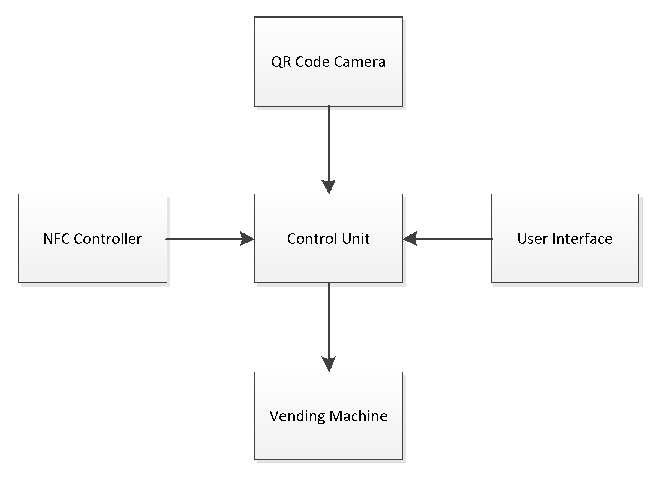
\includegraphics[scale=0.7]{pi_system_overview.eps}
\caption{System overview from the control unit's perspective}
\label{fig:system-overview-pi}
\end{figure}

\begin{figure}[h]
\centering
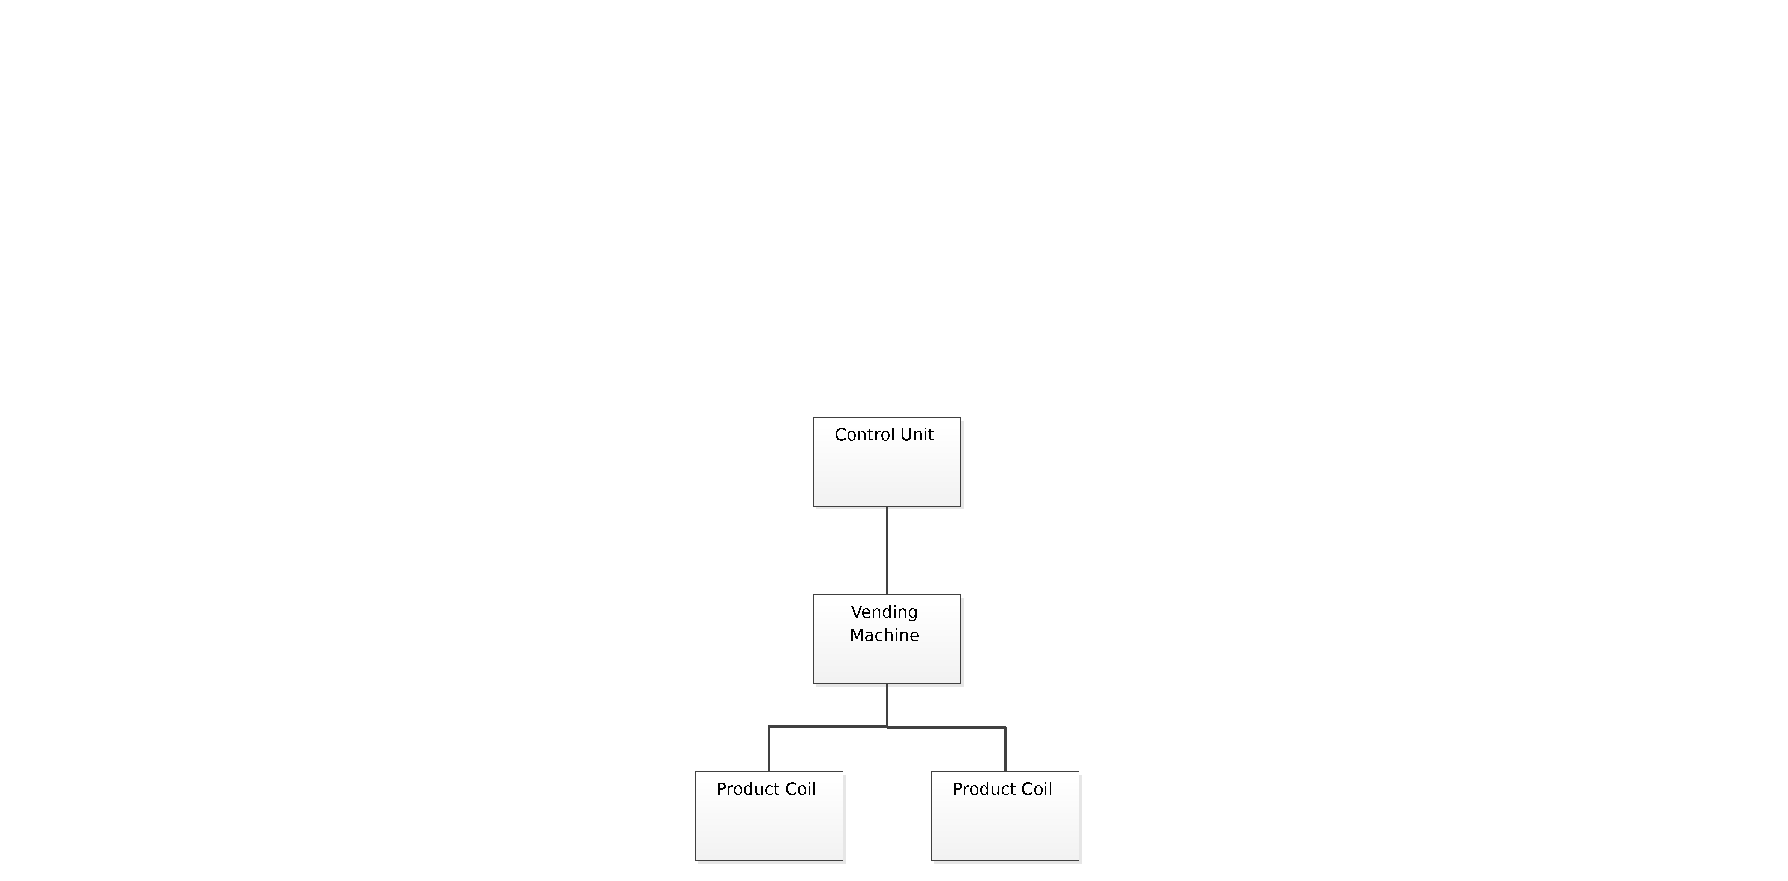
\includegraphics[trim=5cm 0 0 6cm, clip=true,
scale=0.7]{vending_machine_system_overview.eps}
\caption{System overview from the vending unit's perspective}
\label{fig:system-overview-machine}
\end{figure}

It can be seen that the complete system is divided up into five main parts, namely 

\begin{enumerate}
  \item Control unit.
  \item NFC controller.
  \item QR Code camera.
  \item Vending machine unit.
  \item Vending machine coils.
\end{enumerate}

The components used in these subsystems are discussed in the subsequent sections of this
chapter.

\section{Central Control Unit}

To be able to handle the image processing that QR Code decoding and NFC handling requires, a
relatively powerful central controller is required. Although there are many controllers capable
of this, only two main alternatives were considered in this project. They are the Raspberry Pi microcomputer and
the Arduino Uno microcontroller.

\subsection{Arduino Uno}

The Arduino Uno is popular open-source microcontroller (see Figure \ref{fig:arduino}). 

\begin{figure}[h]
\centering
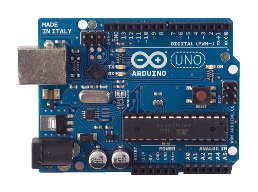
\includegraphics[scale=1.5]{arduino.eps}
\caption[Picture of an Arduino Uno microcontroller]{Picture of an Arduino Uno microcontroller
[\cite{manual:arduino-specs}]}
\label{fig:arduino}
\end{figure}

It is
based on the 8-bit Atmel ATmega328 ARM microprocessor. Its official specifications are [\cite{website:arduino-specs}]:

\begin{tabbing}

Operating Voltage: \= 5 V \\ 
Processor: \> Atmel ATmega328 (clocked at 16 MHz) \\
GPIO Pins: \> 14 (6 of which are PWM enabled) \\
Memory: \> 32 kB Flash, 2kB SRAM, 1kB EEPROM \\
Communication: \> $i^2c$, UART, SPI. \\
Price: \> R310.00 \\

\end{tabbing}

Because of its open-source design, there are a multitude of peripheral devices and expansion
boards (known as `shields'), along with all their libraries and drivers, available locally. The
Arduino's programming language of choice is a modified, but remarkably simple, version of C
and comes with its own Integrated Development Environment (IDE). This, along with its relatively low cost and adequate
specifications, makes the Arduino Uno an attractive option for this project.

\subsection{Raspberry Pi}

The Raspberry Pi is a Debian Linux-based microcomputer
designed and manufactured by a UK-based charity called the Raspberry Pi Foundation, for the
purpose of educating and familiarising young children with programming. However, its low price
and respectable specifications makes it a strong choice for for a control unit for the vending
machine.

The Pi is made with the focus on Python as its main programming language, which makes running
scripts and controlling the board relatively simple. It also runs on a modified version of
Debian Linux called Raspbian.

Its main specifications are [\cite{website:raspi-specs}]:

\begin{tabbing}

Communication: \= SPI, UART, USB, $i^2c$, Ethernet \\ 
Memory: \> 512 MB RAM \\
Processor: \> ARM 6 clocked at 700 MHz \\
Video: \> HDMI video output \\
GPIO: \> 28 pins \\
Price: \> R400.00 \\

\end{tabbing} 

The Raspberry Pi was chosen to be used as the central controller of this project and
controls the hardware connected to it via a Universal Serial Bus (USB) connection, or one of
its General Purpose Input Output (GPIO) pins.

The Pi was chosen instead of the Arduino Uno for the following reasons:

\begin{itemize}
  
  \item The Pi has more processing power (700MHz vs 16MHz).
  \item The Pi's ability to easily interface with desktop computer peripheral hardware,
  such as a keyboard, mouse and webcam.
  \item The excellent support structure in place and the information on existing and ongoing
  projects that are available on the internet.
  \item The Pi can output its video feed to a computer screen, which makes it possible to
  add a simple user interface (GUI) for uder interaction. 

\end{itemize}

Stated simply, the Raspberry Pi is a compact, traditional desktop computer which makes it very
easy to work with, and its low price makes it an excellent choice for use as the central
controller for the vending machine.

\section{NFC Controller}

The NFC controller that was selected is the PN532 NFC shield from Adafruit Industries
[\cite{website:adafruit-nfc}]. It is based on
the Phillips PN532 chip, which is a widely used NFC chip. The main reason it was selected ahead
of other NFC controllers was that it has a large support base in the open source
community and is fully compatible with the libnfc open-source NFC library
[\cite{website:libnfc-hardware}]. The manufacturer (Adafruit, inc.) also provides comprehensive
documentation and guides on how to set up and configure the controller.
 
The main purpose of this component is to add the option of sending or receiving data through a NFC connection.
This component is also capable of reading RFID cards, such as student or staff cards, as NFC
and RFID transmit similar types of data. This adds the option of paying for the products with 
any NFC-capable smart phone running Google's Android operating system, or with a SU staff or
student card.

\section{QR Code Camera}

To decode QR Codes, the vending machine needs to take pictures of a code so that it can be
decoded using the ZBar library. A PlayStation 2 EyeToy was chosen and added to the system to
facilitate this. It was chosen for the following reasons:

\begin{itemize}
  \item Its drivers are freely available for Linux systems [\cite{website:webcam-drivers}].
  \item Interfaces easily with the USB ports on the Pi.
  \item There was one lying in the supply cupboard.
\end{itemize}

There is currently a camera add-on available for the Raspberry Pi, but this is relatively
expensive and (approximately \$30 [\cite{website:raspi-camera}] versus the Pi's \$35), at the
time of writing, unavailable in South Africa.

\section{Product Dispensing}

\subsection{Coils}

To be able to effectively dispense bought products to the user, a traditional coil mechanism is
used. Such systems are the most familiar and simple methods of dispensing goods. See Figure
\ref{fig:vm-coils} for an example.

\begin{figure}[h]
\centering
\includegraphics[scale=0.2]{vm_coils.eps}
\caption{Example of vending machine coil system [\cite{website:arduino-specs}]}
\label{fig:vm-coils}
\end{figure}

These coils are designed and made in such a manner that one rotation of the coil will drop one
product. The turning motion is made by attaching a DC motor to the base of the coil (see
section \ref{sec:dc-motor} for a more detailed description).

\subsection{DC Motors}
\label{sec:dc-motor}

The motors attached to the base of the coils are two 12V DC mootors from Faulhaber
[\cite{manual:dc-motors}]. Although these motors are rated for 12V, it is possible to run them
from a lower voltage. This will cause the motor to turn slower, and therefore be easier to
control. 

The motors are switched on by a 12V relay switch controlled by the Raspberry Pi. See section
\ref{sec:relay-switch} for more detail about the switch.

\subsection{Relay Switch}
\label{sec:relay-switch}

A relay is a type of electronic switch, which means that it acts like a normal switch, but
requires a voltage across it to open or close it. With this it is possible to control when the
DC motors turn (after a successful transaction) and when they are standing still. 

However, the relays used here are 12V. The Raspberry Pi can deliver a maximum of 5V. Therefore
it was decided that the relay will be permanently connected to a 12V DC supply, but will be
switched by a 2N2222 transistor, which is controlled directly from the Pi's  GPIO pins (see
section \ref{sec:detail-switch} for a detailed discussion).

This allows the Pi to directly control the motors and due to the circuits construction, the Pi
is protected from the relatively high voltages and currents involved in the working of the
motor nd relay.

\section{Vending Machine Unit}

The vending machine unit houses all the components (i.e. the Raspberry Pi, the NFC Shield,
webcam, switches, motors and the product coils). Its made of 1.6mm mild steel plate and was
made by Fabrinox, Paarl. See Appendix \ref{app:vm-tekeninge} for detailed manufacturing
drawings.

\chapter{Software Detail Design}

In this chapter, the software design aspects of this project are discussed in
detail.

This chapter is divided up into four sections, with each section explaining what
the program being discussed is responsible for, what third party programs it
uses and how it interacts with the rest of the system. 

These four sections are:

\begin{enumerate}
  \item The security scheme used.
  \item The web server that was created.
  \item The vending machine's control program.
  \item The Android app that was created.
\end{enumerate}

\section{Security Scheme}
\label{sec:security-code-scheme}

In addition to the asymmetric encryption used on all data transfer to and from
the server to its clients, two more layers of security were added to prevent
repeated use of the same code and to make it harder for hackers to crack the
encryption key.

\subsection{Random Character String}

The product code transmitted to the server is embedded inside a
random 16-character string of hex values, i.e. numbers from 1 to 9 or characters
from A to F. The product code is a 4 character hex string, but this is saved on
the database and can therefore not be random. 

This is done to prevent any would-be
hackers from realising that they have cracked the system's encryption. In other
words, if the hackers have cracked the encryption, they will still see 16
random hex characters and think that the encryption is still intact.

\subsection{Challenge and Response Code}

The second layer of security added is a challenge/response system. Such a system
works by having party A generate a challenge (this can be a string or a number).
Party B then takes this challenge and puts it through a previously agreed-upon
process, e.g. makes the letters capital or adds the numbers together. This
is the response. Party B then sends the back the response to party A, which then
checks to see if its a valid response to party A's original challenge.

In the case of the vending machine, a 16 character hex string is being
generated. It was decided to use 4 characters of this random string as the
vending machine's challenge. After receiving this challenge, the server then
takes out the agreed-upon 4 characters and adds it to the server's response
code. When the vending machine scans the customer's response QR Code, the
vending machine checks to see if the 4 character response was part of its
original code the vending machine generated.

This system is used to prevent customers from only buying one product and using
the same code again to get another product for free. Thus, the
challenge/response code system makes each code only valid for one transaction.

\section{Web Server Program Design}

The web server that was made for this project is based on the Django web framework for Python
(see Section \ref{sec:django} for some background information). The Django server was then
configured to run on top of an Apache web server located on an Amazon Web Service (AWS) Elastic
Compute Cloud (EC2) cloud computer instance (see Section \ref{sec:ec2} for some background
on EC2 and Section \ref{sec:apache} for some background on Apache).

The server is responsible for handling all the data and financial transactions that will take
place during the vending machine's operation. 

This section stipulates the design of the complete server and how the different components
interact with one another. 

\subsection{Django Server}

The Django server is responsible for all of the scripting and database work that the server
performs. The server is divided up into a total of six applications. Each of these is
responsible for either displaying a single web page or to handle data requests from the
Near Field Communication (NFC) Android app (see Section \ref{sec:nfc-android-app} for more
details).

The website apps and their interactions with the real world and one another
are given in Figure \ref{fig:website-apps}. 

\begin{figure}[h]
 \centering 
 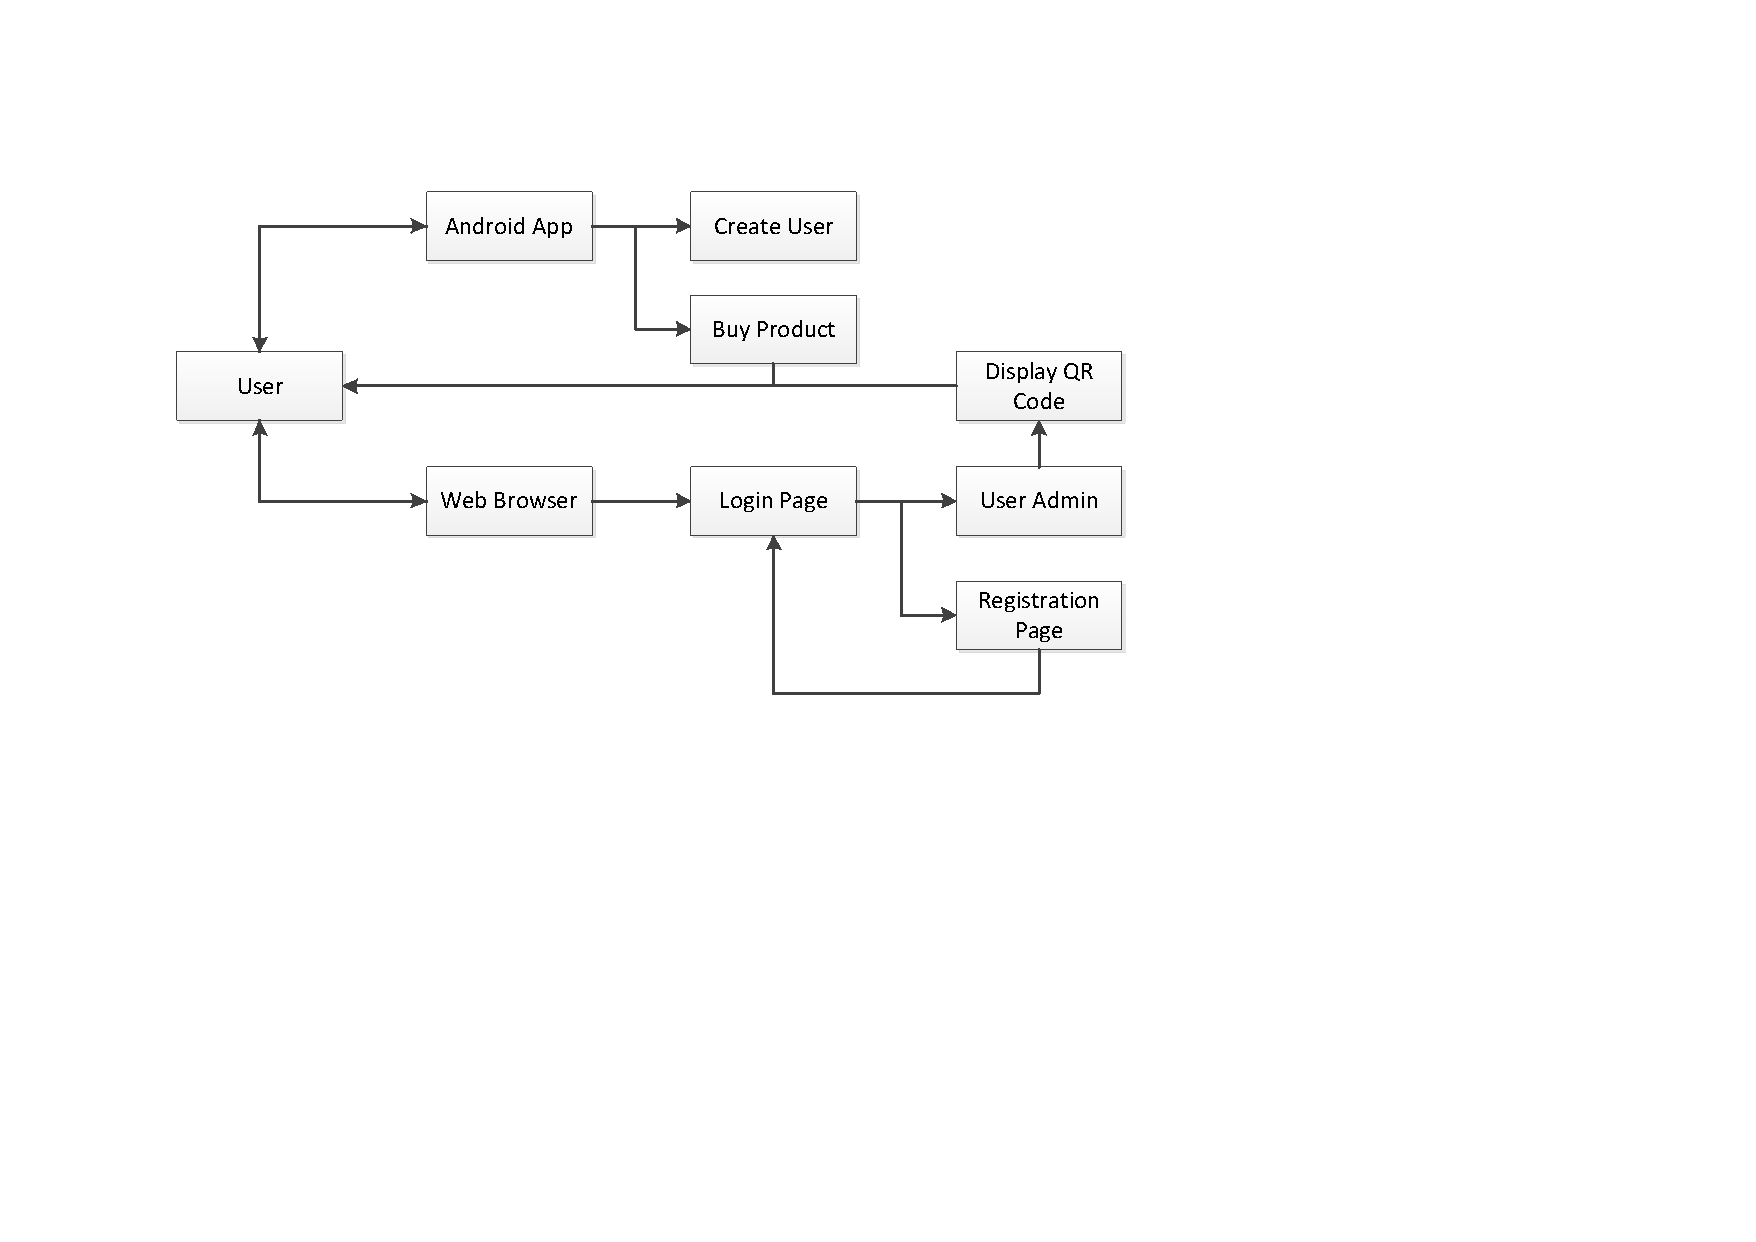
\includegraphics[clip=true, trim = 0 130 130 30,
 scale=0.7]{website_structure}
 \caption{The web server app structure}
 \label{fig:website-apps}
\end{figure}

\subsubsection{display\_qrcode}

This app forms the core of the Quick Response Code (QR Code) payment handling part of the
server. See Figure \ref{fig:disp-qrcode} for the process flow of this app.

\begin{figure}[h]
 \centering 
 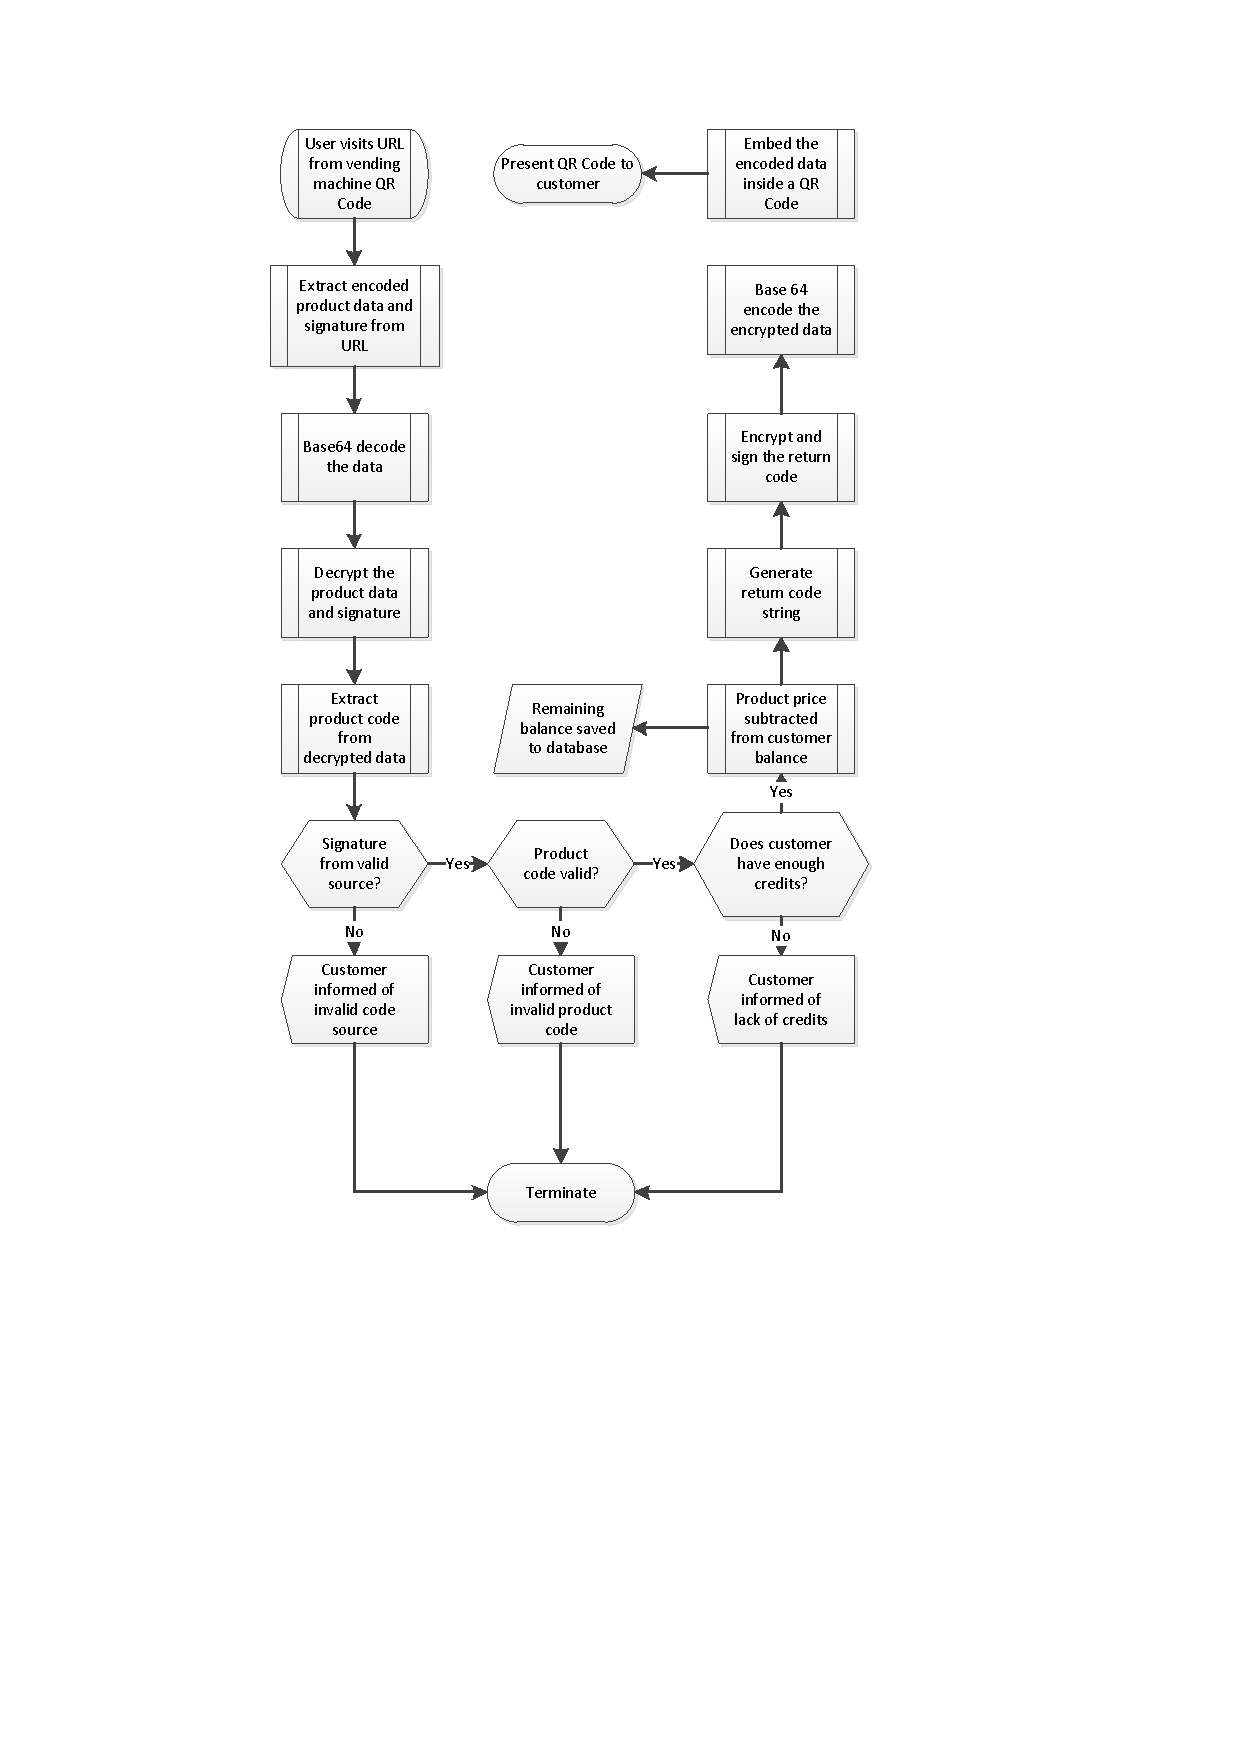
\includegraphics[clip=true, trim = 0 250 0 50,
 scale=0.7]{qrcode_processflow_server_bak}
 \caption{The display\_qrcode app process flow}
 \label{fig:disp-qrcode}
\end{figure}

As seen from Figure \ref{fig:disp-qrcode}, the app first extracts the code containing the
product code and vending machine's signature from the Uniform Resource Locator (URL) that the
customer visited with his/her cell phone's web browser. The app then proceeds to decode the
the code from the base64 encoded format it was sent in (see Section \ref{sec:base64} for some
background information on base 64 encoding).

After successfully decoding the data, the app proceeds to decrypt the data and signature with the ElGamal
algorithm using the server's private key and the vending machine's public key
(see Section \ref{sec:assymetric-encryption} for more detail on public and private keys) and, following the
security code scheme described in Section \ref{sec:security-code-scheme}, extracts the product
code from the decrypted string.

The app then checks to see if the signature comes from a valid source (i.e. one of the vending
machines using this system), if the product code is valid (i.e. the product is in the database)
and if the customer has enough credits loaded loaded onto his/her account. If either of these
checks return false, an appropriate error message is shown to the customer explaining what
went wrong and what the customer should do next.

If the checks were passed, the app proceeds to subtract the product cost from the user's
remaining balance. Using the security code scheme, the app then generates the correct return
code, encrypts and signs it with the vending machine's public key and the server's private key,
and encodes it with base 64. After this is completed, the app embeds this data into a QR Code,
which is returned to the customer's cell phone screen. 

\subsubsection{load\_money}

This app allows the customer to load money onto his/her account. At the moment it makes use of
faux money, meaning that the money loaded has no real-world value. The customer can load a
maximum of R1000.00 onto his/her account.

See Figure \ref{fig:load-money} for the process flow of this app.

\begin{figure}[h]
 \centering 
 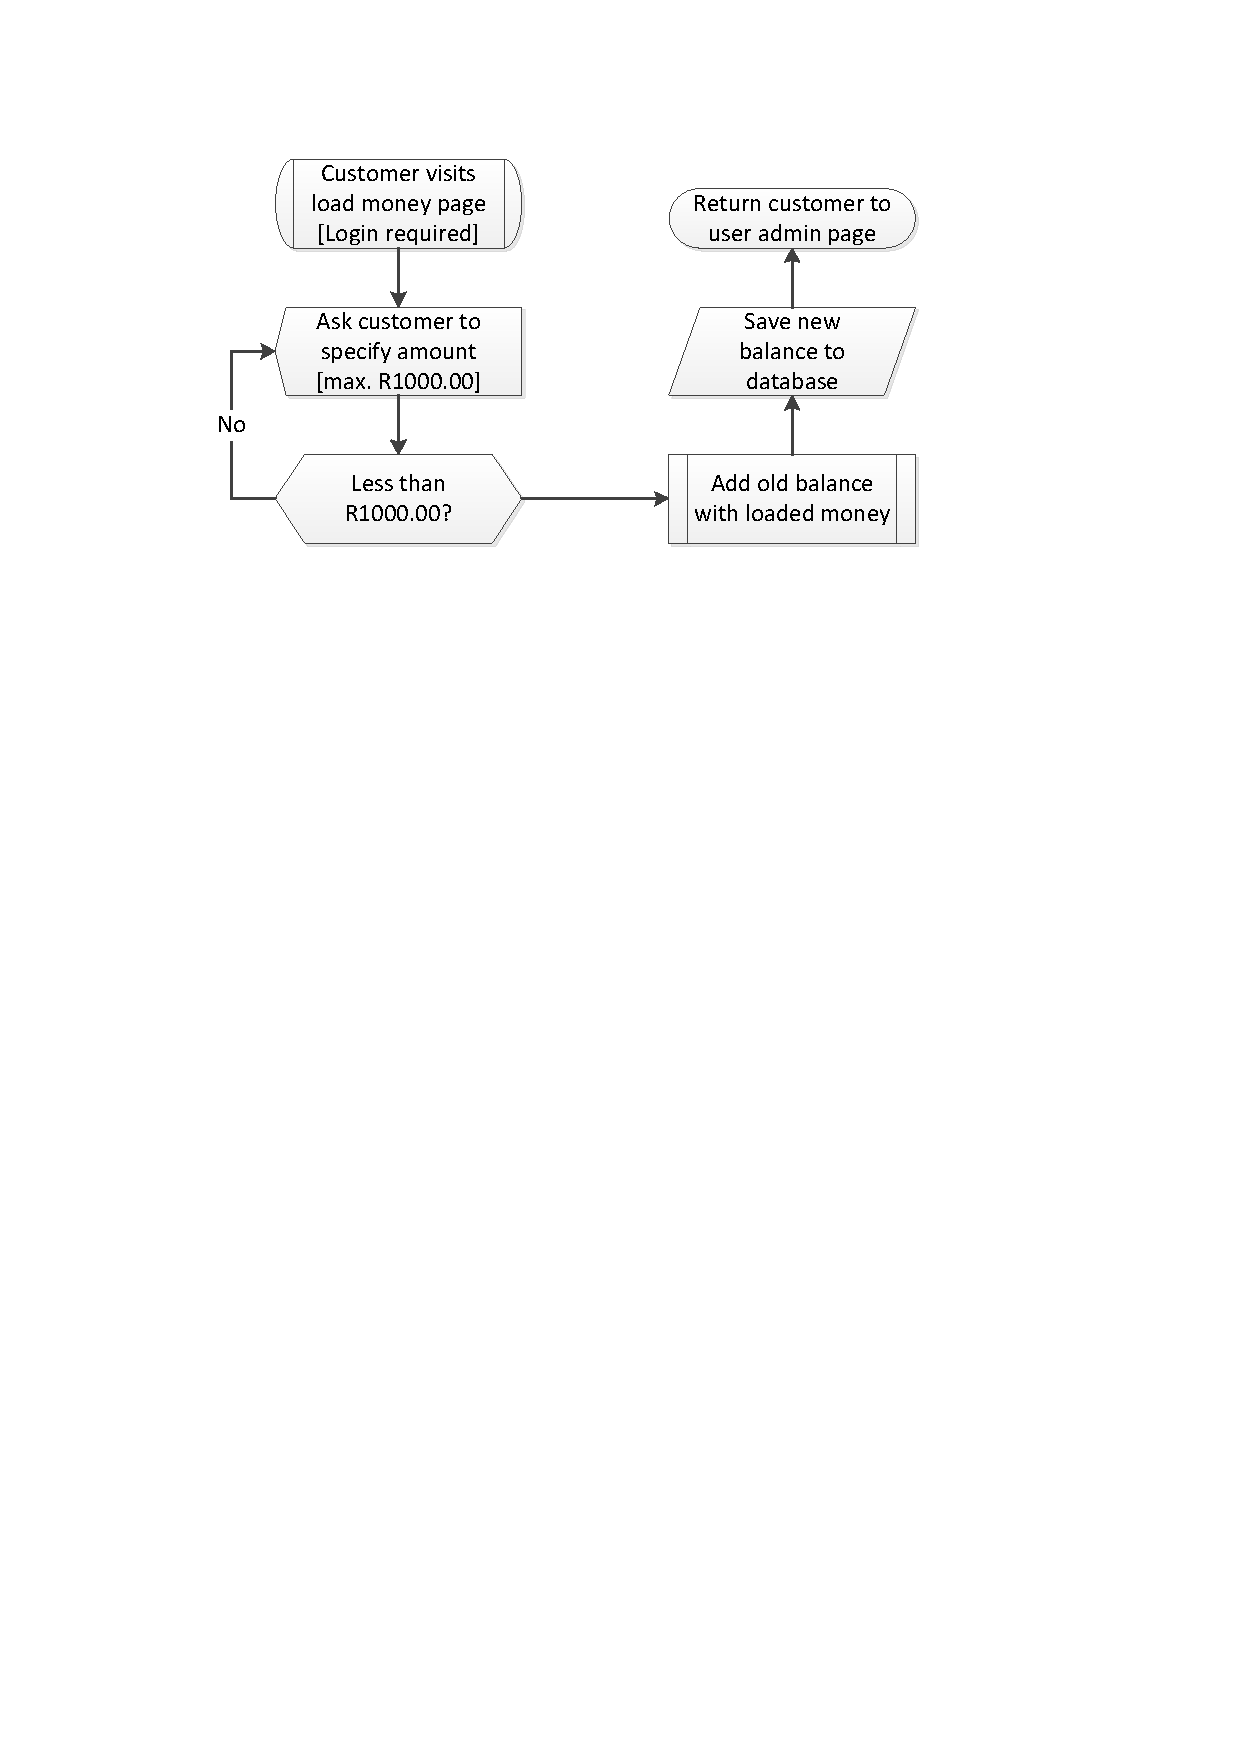
\includegraphics[clip=true, trim = 0 580 100 60,
 scale=0.7]{load_money}
 \caption{The load\_money app process flow}
 \label{fig:load-money}
\end{figure}

\subsubsection{nfc}
\label{sec:app-nfc}

This app forms the core of the NFC payment handling part of the server. See Figure
\ref{fig:nfc-process} for a detailed process flow diagram.

\begin{figure}[h]
 \centering 
 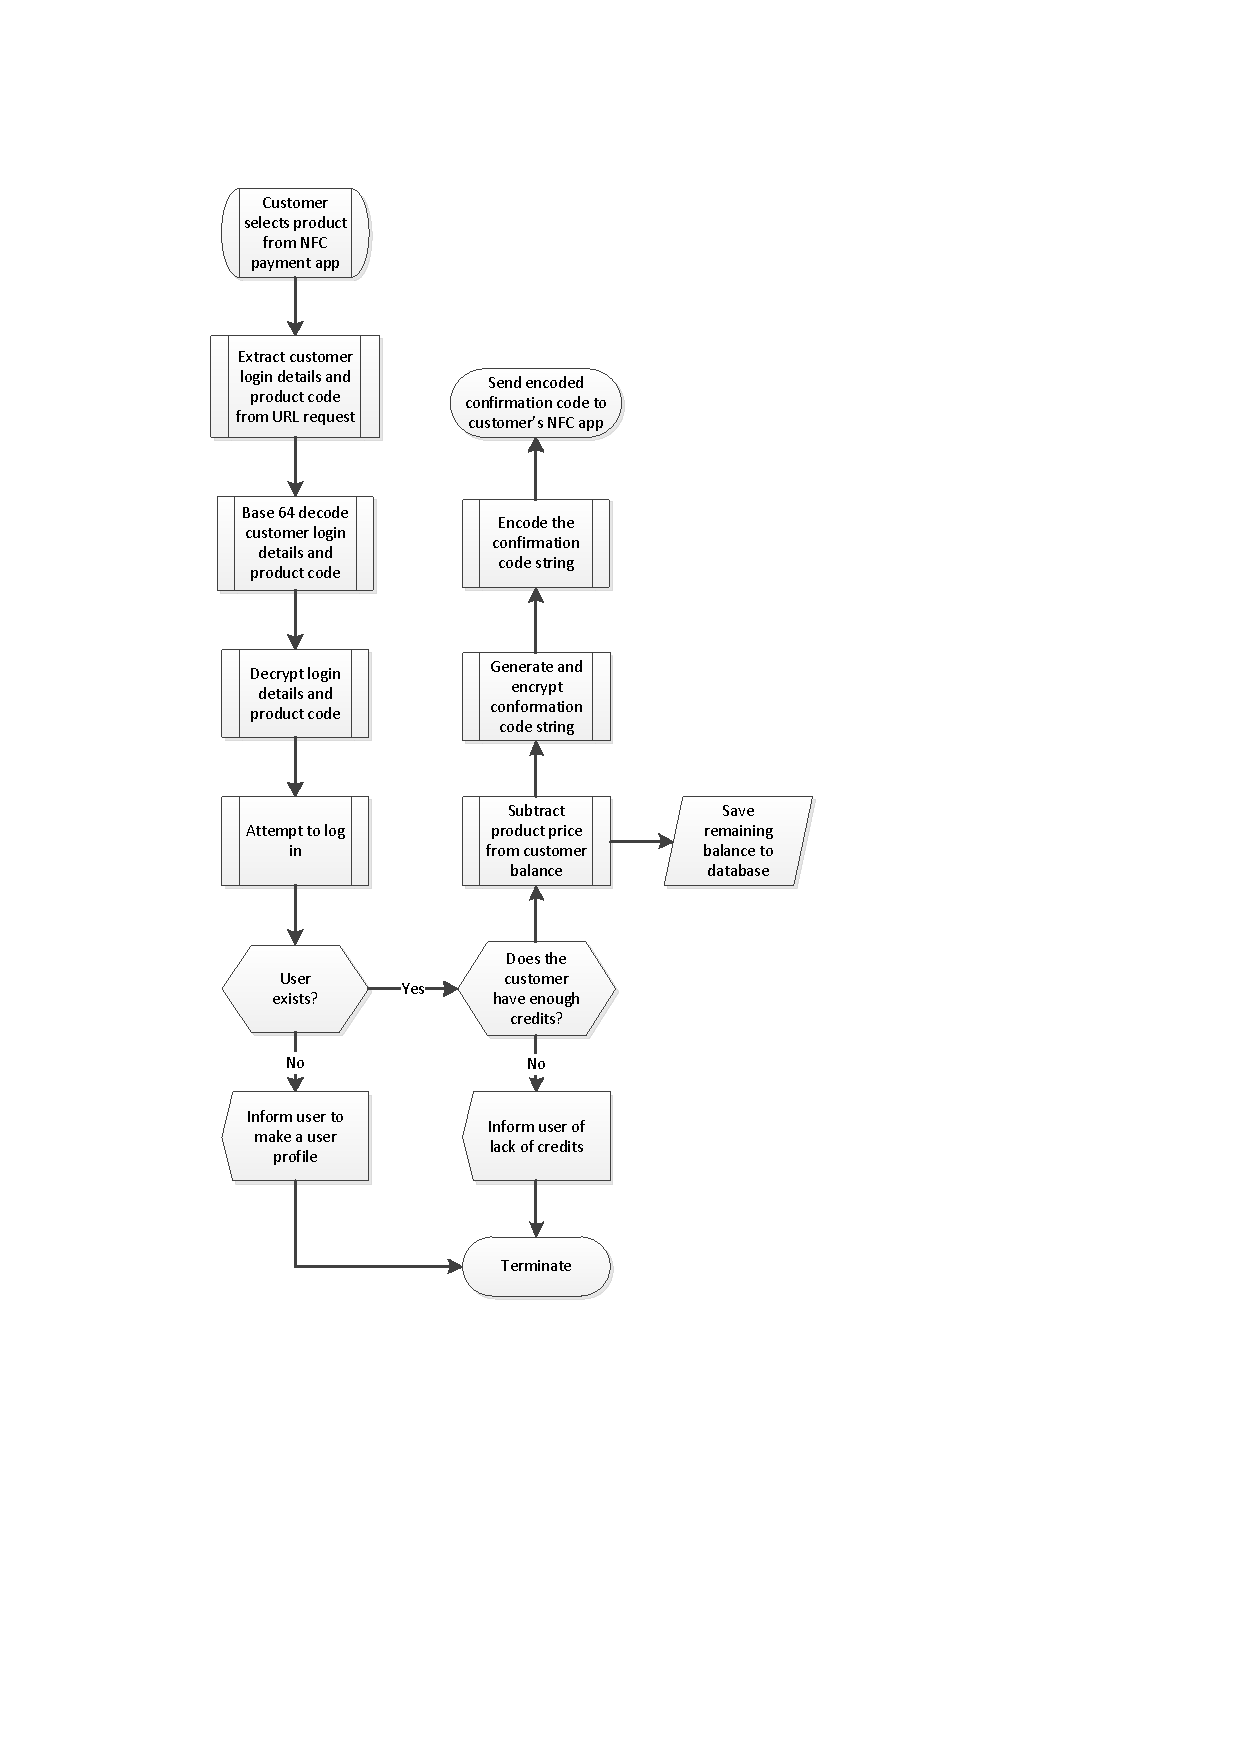
\includegraphics[clip=true, trim = 0 200 100 80,
 scale=0.7]{nfc_processflow_bak}
 \caption{The nfc app process flow}
 \label{fig:nfc-process}
\end{figure}

As seen from Figure \ref{fig:nfc-process}, the server first extracts the encoded and encrypted
customer login details and product code from the URL the NFC app sends to the server. These
codes are then all decoded and decrypted using the Ron Rivest, Adi Shamir and Leonard Adleman
(RSA) algorithm and the server's private key. 

The user login details are then checked and verified using the server's user database. If this
check fails, the customer is given an appropriate error message and informed to create a user
profile. 

If the check is passed, the server then checks to see if the customer has enough money loaded
onto his/her account. If this check fails, the customer is informed of his/her lack of funds
and is instructed to load more money. If the check is passed, the server subtracts the product
cost from the customer's balance and encrypts and encodes a confirmation code, according to the
security code scheme specified in Section \ref{sec:security-code-scheme}, which is then sent
to the NFC app. 

\subsubsection{nfc\_add\_user}

This app allows a customer using the NFC app to create a user profile for himself/herself. The
server extracts the customer's login details from the URL request that the NFC app send to the
server. The user name and email are kept in plain text, but the password is decrypted to
plain text with the RSA algorithm and the server's private key.

These details are then saved to the database and is immediately available to be used by the new
customer. 

\subsubsection{register}

This app allows a new customer to register. This app is only accessible by a web browser and
not by the NFC app. However, a user registered with this app will be able to use the same login
details for the NFC app.

The app presents the user with a simple registration page which asks for a user name, email and
password. Using Django's built-in form support. This allows the server to handle the
POST request that is generated when the customer presses the `Continue' button. When this is
done, the login data contained within the POST request is extracted and saved into the user
database. 

\subsection{EC2}

The AWS EC2 server provides the platform on which the Apache server runs. The EC2 server
instance was configured to run Ubuntu 12.10, `Quantal Quetzal'. This was done because most of
the server development was done on Ubuntu 12.10, and the server code will therefore require
minimal adaptation to be able to run on the EC2 server. 

After the server instance was created, the following packages and programs were installed for
the server to be able to run properly:

\begin{itemize}
  \item Apache2: Installs the Apache server framework.
  \item libapache2-mod-wsgi: An Apache module that allows Apache to work with Python wsgi
  scripts.
  \item python-pip: Allows Ubuntu to install Django from the Python Package Index (PyPI)
  [\cite{website:pypi}].
  \item Django: Installs the all the Django packages that will be used by the server. 
\end{itemize}

Because the server's database uses SQLite3, and Ubuntu 12.10 comes with it by default, no
external database programs were needed to be installed. 

After this was completed, the server is fully capable of serving Django web
pages.

\subsection{Apache}

The Apache server framework provides the foundation on which the Django server runs. It had to
be configured to be able to run the Python scripts that Django contains. To do this, the steps
described in Nick Polet's blog post was followed [\cite{article:apache-setup}]. It describes
in detail how to configure Apache to serve a Django website.

For Apache to be able to serve Django sites, it had to be configured to run the Web Server
Gateway Interface (wsgi.py) script located within the Django server folder. This was done by
adding the following code to the Apache's httpd.conf configuration file:

\begin{verbatim}
WSGIScriptAlias / /home/ubuntu/srv/server_site/server_site/wsgi.py
WSGIPythonPath /home/ubuntu/srv/server_site

<Directory /home/ubuntu/srv/server_site/server_site>
<Files wsgi.py>
Order deny,allow
Allow from all
</Files>
</Directory>
\end{verbatim}

The following line was also needed to be added to Apache's apache2.conf file:

\begin{verbatim}
Include httpd.conf
\end{verbatim}

\section{Vending Program}

The vending machine's program runs the vending machine. Its responsible for
allowing the customer to select a product, to create a QR Code for that points
takes the customer to the web server, to scan the customer's response QR Code,
to scan the customer's NFC request and to dispense the product after a
successful transaction. The whole program is based on Python scripts and
designed to be used by a Raspberry Pi microcomputer (see Section
\ref{sec:raspi} for more details).

To simplify the program, its split up into separate sub-programs. These
sub-programs, called scripts, are discussed in this section.

\subsection{User Interface}

To allow the customer to select a product, a Graphical User Interface (GUI) was
created. The GUI was made using the WX Python GUI toolkit
[\cite{website:wx-python}].
See Figure \ref{fig:gui-screenshot} for a screenshot of the GUI and Figure
\ref{fig:gui-processflow} for the GUI process flow.

\begin{figure}[h]
 \centering 
 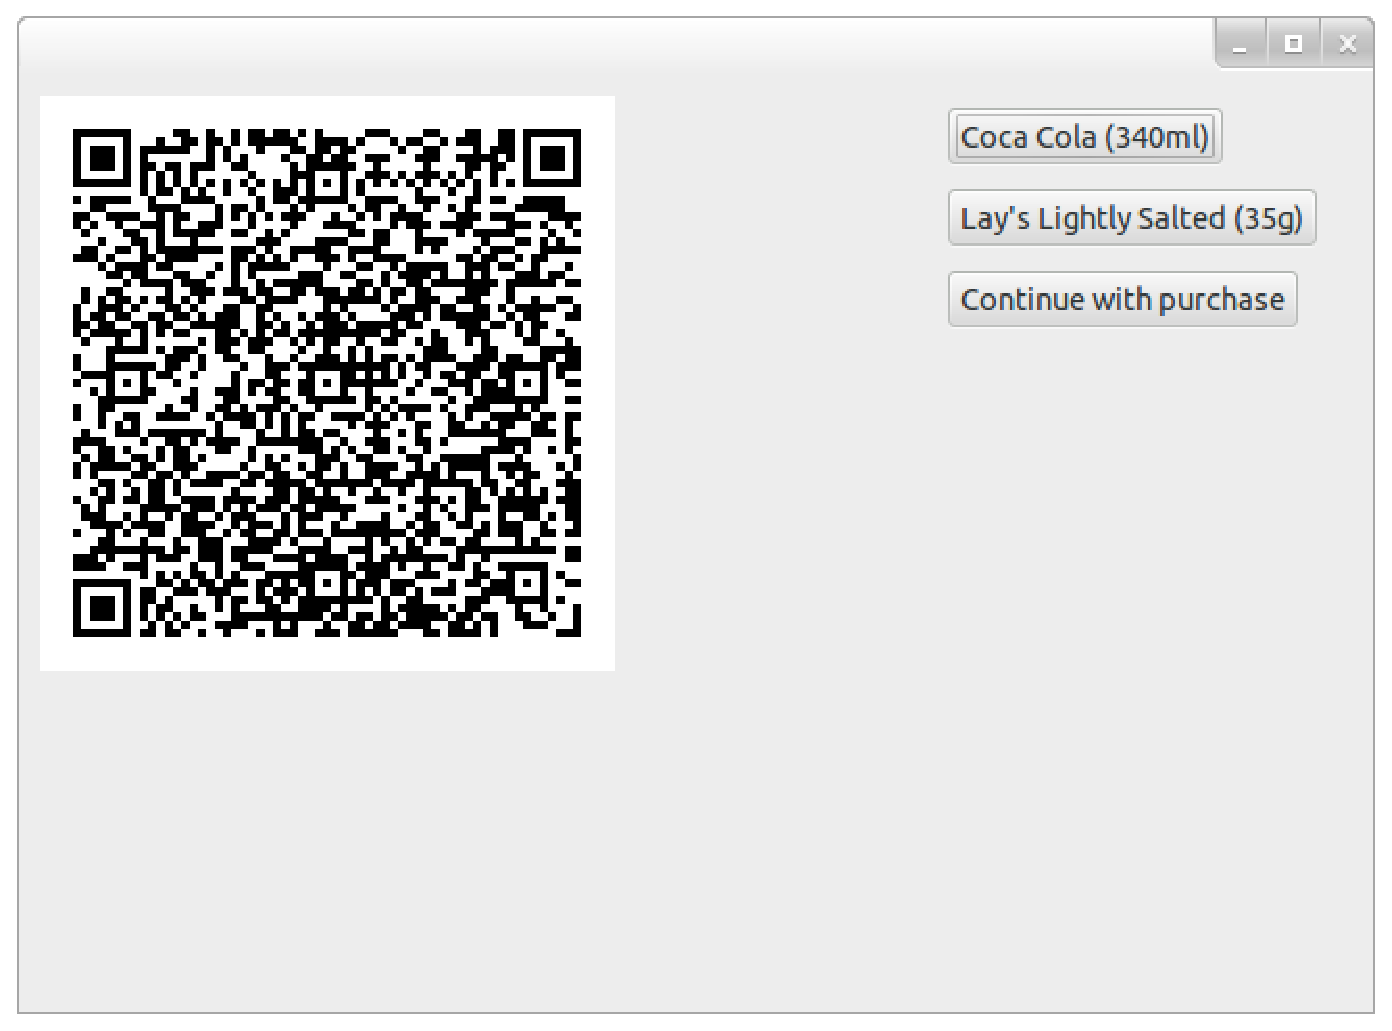
\includegraphics[scale=0.4]{gui_screenshot}
 \caption{A screenshot of the user interface}
 \label{fig:gui-screenshot}
\end{figure}

As can be seen from Figure \ref{fig:gui-processflow}, the GUI script is
responsible for calling the encryption script and the QR Code generation script.
It is also responsible for displaying the QR Code, to handle transactions from
the Android NFC app and to activate the correct motor inside the vending
machine. 

\subsection{Generate Product Code}

After the customer selects which product to buy from the GUI, the
encrypt\_elgamal script is called. This script is responsible for generating the
random hex character string, in accordance with the security scheme described in
Section \ref{sec:security-code-scheme}, encrypting, signing and encoding the
string in base 64 and embedding the random string inside a Uniform
Resource Locator (URL) that points to the web server. This URL is then sent to
the generate\_qrcode script described in Section \ref{sec:generate-qrcode}.

See Figure \ref{fig:gen-prod-code-processflow} for a detailed process flow
diagram.

\subsection{Generate QR Code}
\label{sec:gen-qrcode}

After the encrypt\_elgamal script has been run, the generate\_qrcode script is
called. This script is responsible for embedding the URL received from the
encrypt\_elgamal script into a QR Code. This is done by using a qrcode module
for Python, called qrcode [\cite{website:qrcode-generator}].

\subsection{Read QR Code}

After the customer has received his/her QR Code from the server verifying the
transaction, the customer may press the button called `Continue with purchase'.
When this is done the read\_qrcode script is run.

This script is responsible for reading the customer's QR Code via a web cam,
extract the data from the scanned image, decrypting the data and verifying the
transaction. See Figure \ref{fig:read-qrcode-processflow} for a detailed process
flow diagram. 

As seen from Figure \ref{fig:read-qrcode-processflow}, as soon as the `Continue
with purchase' button is pressed, the script creates a ZBar image processor
which scans a web cam video feed for a QR Code (see Section \ref{sec:zbar} for
more information on ZBar). This image processor runs until the user cancels the
process or it scans a QR Code. 

After the ZBar processor has scanned a QR Code, it sends the retrieved data to
be decrypted and verified with the ElGamal algorithm and the vending machine's
private key and the server's public key. If the signature is valid and the data
contains a valid response and product code, the script activates the correct
motor and the customer receives his/her product. 

\subsection{Near Field Communication}

If the customer opts to purchase a product with the Android Near Field
Communication (NFC) app, the NFC script is run. This script is based on an
example script included in the nfcpy package (see Section \ref{sec:nfcpy} for
more detail) and is written by nfcpy's creator, Stephen Tiedemann
[\cite{website:nfcpy}]. This example script, called snep-test-server, does the
following:

\begin{itemize}
  \item It connects the Raspberry i to the NFC controller chip.
  \item It polls the NFC controller chip for a Simple NFC Data Exchange Format
  Exchange Protocol (SNEP) message.
  \item When a SNEP message is read, it extracts the data in the message and
  presents it to the programmer for further processing and manipulation.
\end{itemize}

Using this example script allows the vending machine to extract SNEP messages
from any source that follows the NFC Forum's standards
[\cite{website:nfc-forum}]. For this project, an Android NFC app was written
specifically for this purpose (see Section \ref{sec:nfc-android-app} for more
detail). 

After the data is extracted from the NFC source, the script decrypts the data
using the RSA algorithm and the vending machine's private key. The vending
machine then checks the NFC message's response code. 

If the response code is valid, the script then activates the correct motor to
dispense the product to the customer.

\section{Android app}
\label{sec:nfc-android-app}

An Android NFC app was made for this project. It allows a customer to buy a
product from the app's product menu and to complete the purchase by swiping
his/her phone across the vending machine's NFC receiver.

The app is divided up into three activities (Android's technical term what what
is essentially a different window of the app). 

These activities, their design and significance are discussed in this section.

\subsection{Welcome Screen}

This activity is the activity that is called when the app is opened. This
activities process flow can be seen in Figure \ref{fig:app-welcomescreen}.
Figure \ref{fig:welcomescreen-screenshot} shows a screenshot of the welcome
screen.

\begin{figure}[h]
 \centering 
 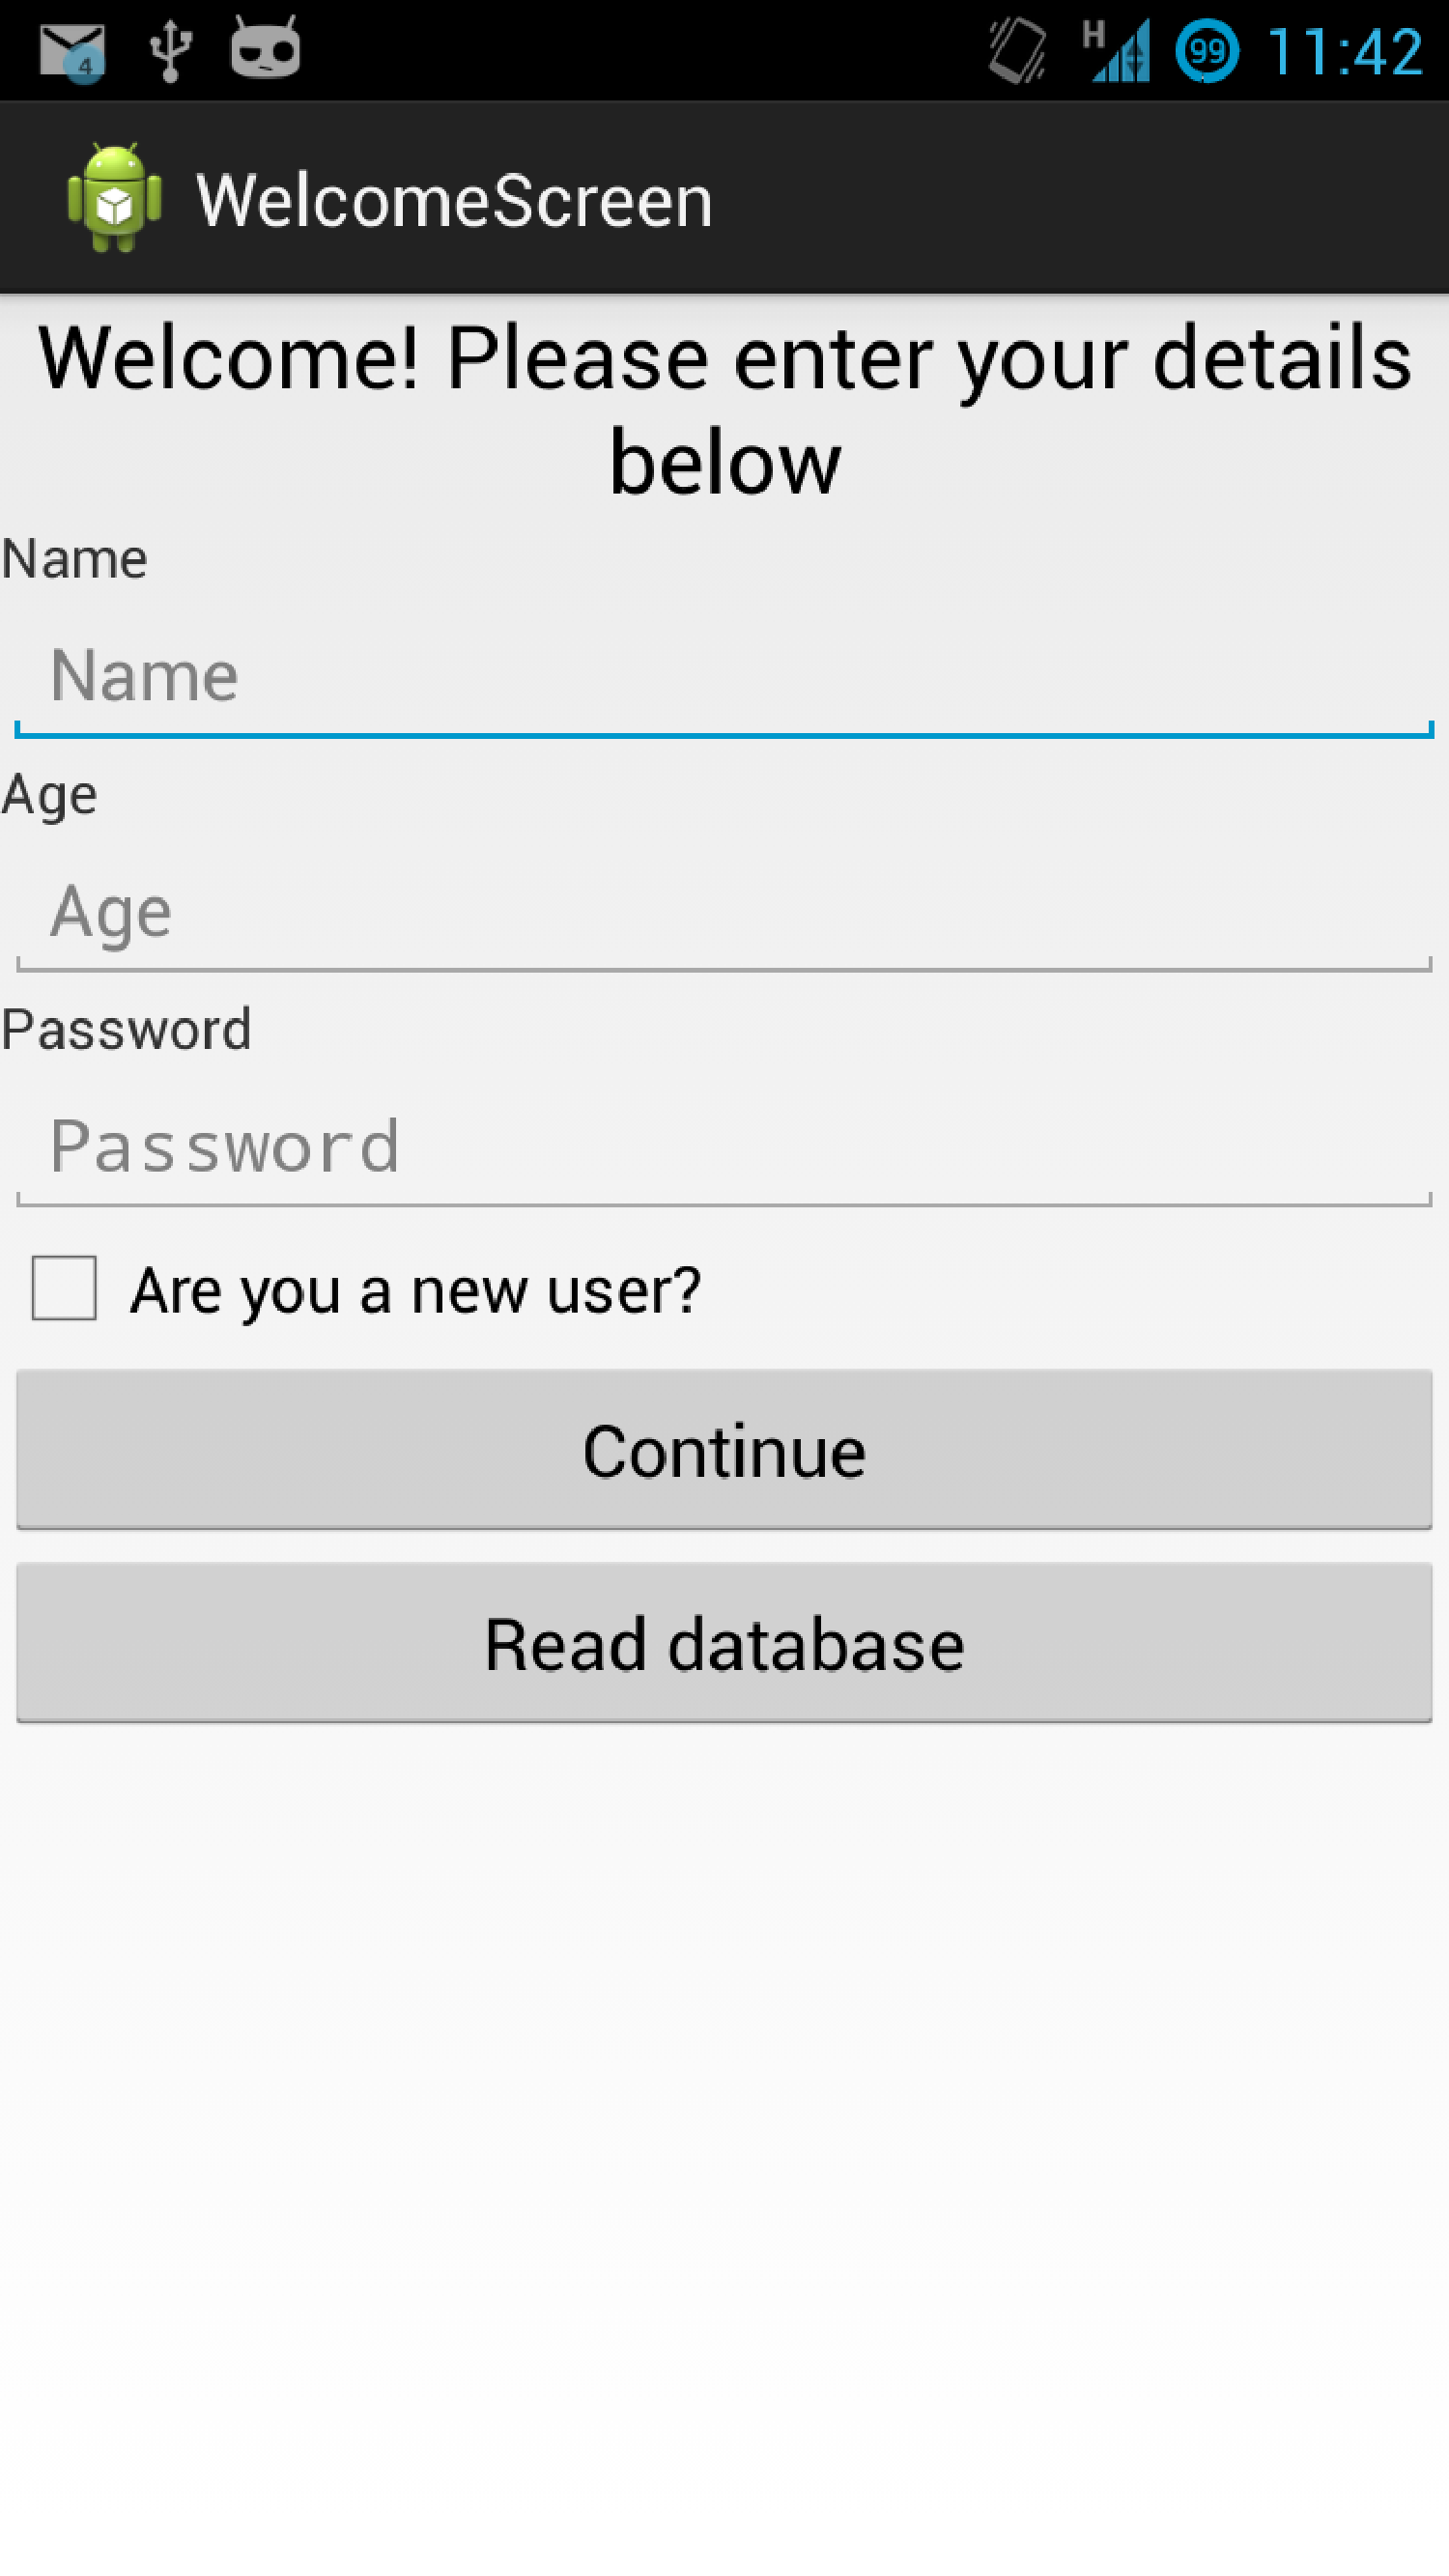
\includegraphics[clip = true, trim = 0 320 0 60, scale=0.2]{welcome_screen}
 \caption{A screenshot of the app's welcome screen}
 \label{fig:welcomescreen-screenshot}
\end{figure}

As seen from Figure \ref{app-welcomescreen}, the activity first checks to see
if its the first time the user opens the app. If its not, the activity goes on
to the Main Activity. Otherwise, it allows the user to either sign in with an
existing profile or create a new one.

When the user signs into an existing profile, the login details he/she provides
is stored in a database that is only accessible by this app. This is done he
data is saved to a database to make it persistent throughout the lifetime of the app

These details are also saved into an app-wide variable. This variable is
only accessible by the app and is only active while the app is running in
the foreground or background. This variable is used to make the app more
efficient by not having to read the database every time the user wants to use
the app. This variable is only active while the app is running in the foreground
or background

The login details saved here are used later by the app's other activities.

\subsection{Change User Settings}

The Change User Settings activity allows the user to change his/her login
details that are saved in the database and the app-wide variable. See Figure
\ref{fig:change-user-settings} for a detailed process flow diagram for this
activity. Figure \ref{fig:change-settings-screenshot} shows a screenshot of this
activity.

\begin{figure}[h]
 \centering 
 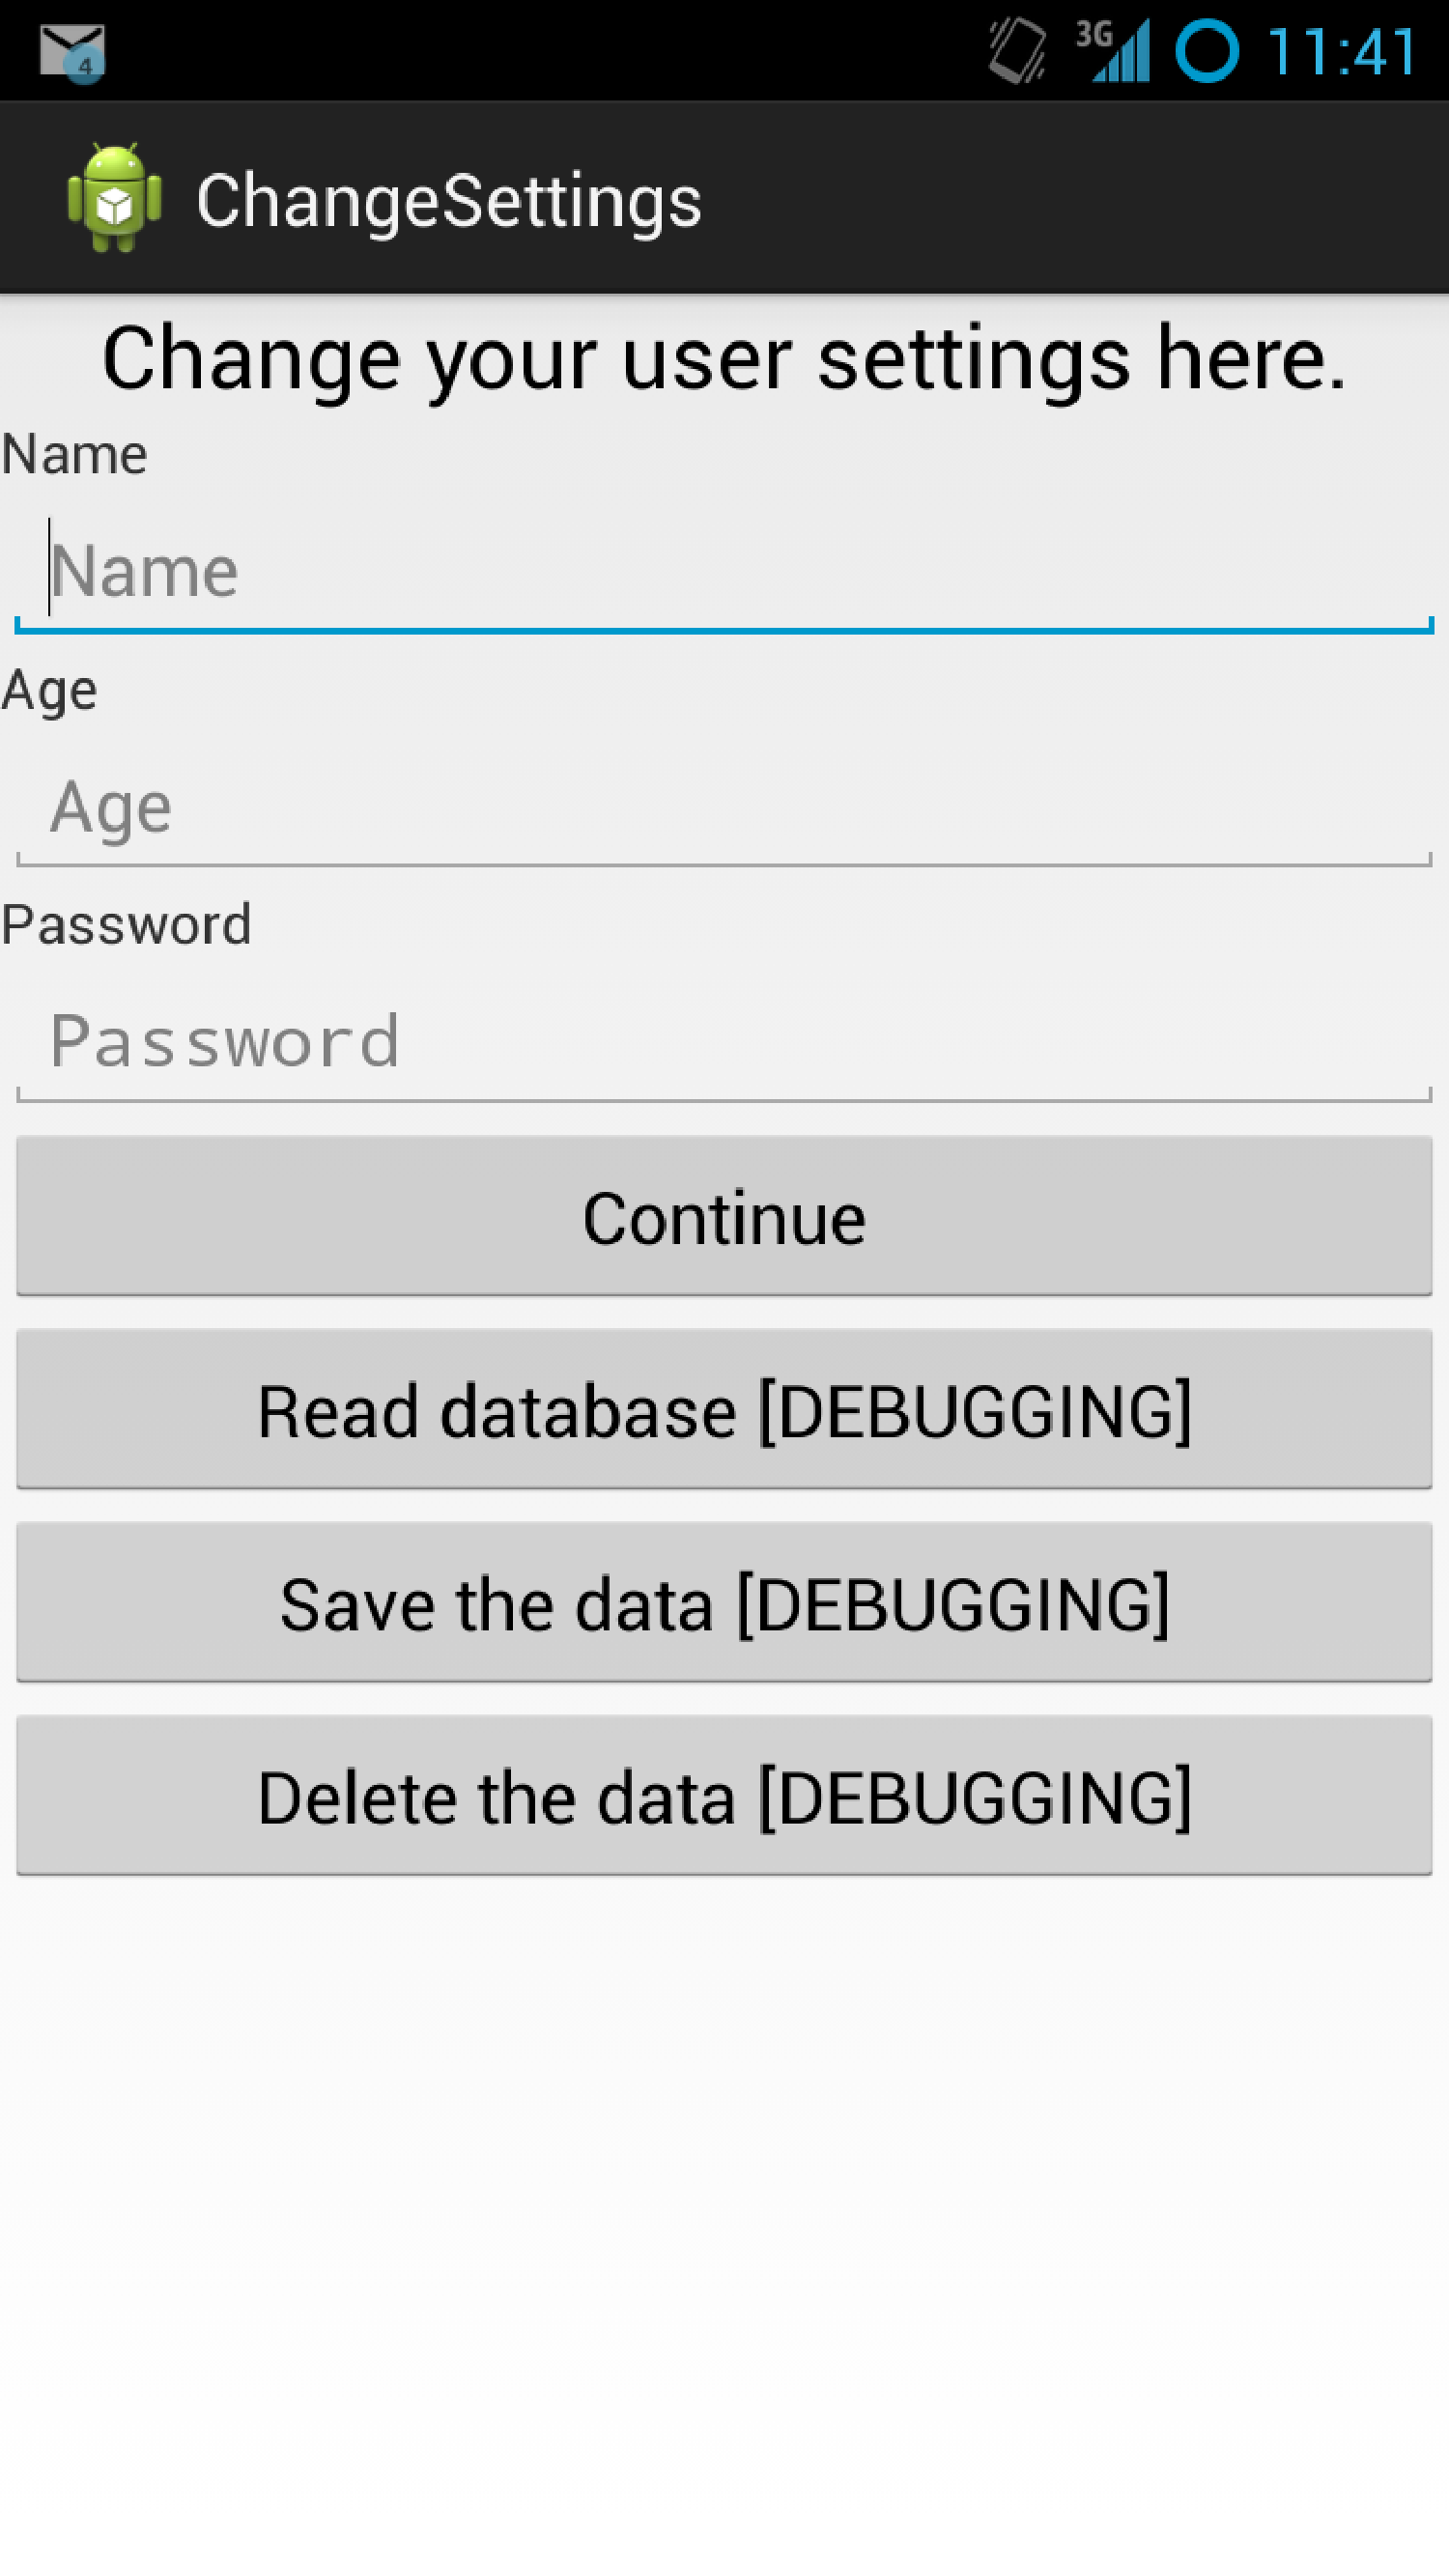
\includegraphics[clip = true, trim = 0 320 0 60,
 scale=0.2]{change_settings}
 \caption{A screenshot of the app's change settings activity}
 \label{fig:change-settings-screenshot}
\end{figure}

When the app enters this activity, it prompts the user to enter his/her user
name and password. When the user presses the `continue button', the old database
entry and app-wide variable is overwritten with the new values the user entered.

\subsection{Main Activity}

The main activity is the activity which is responsible for encrypting and
sending the purchase requests to the web server, receiving and decrypting
the purchase approval codes and sending the NFC messages to the vending machines
NFC receiver. See Figure \ref{fig:main-activity} for a process flow diagram
and Figure \ref{fig:main-activity-screenshot} for a screenshot of this activity.

\begin{figure}[h]
 \centering 
 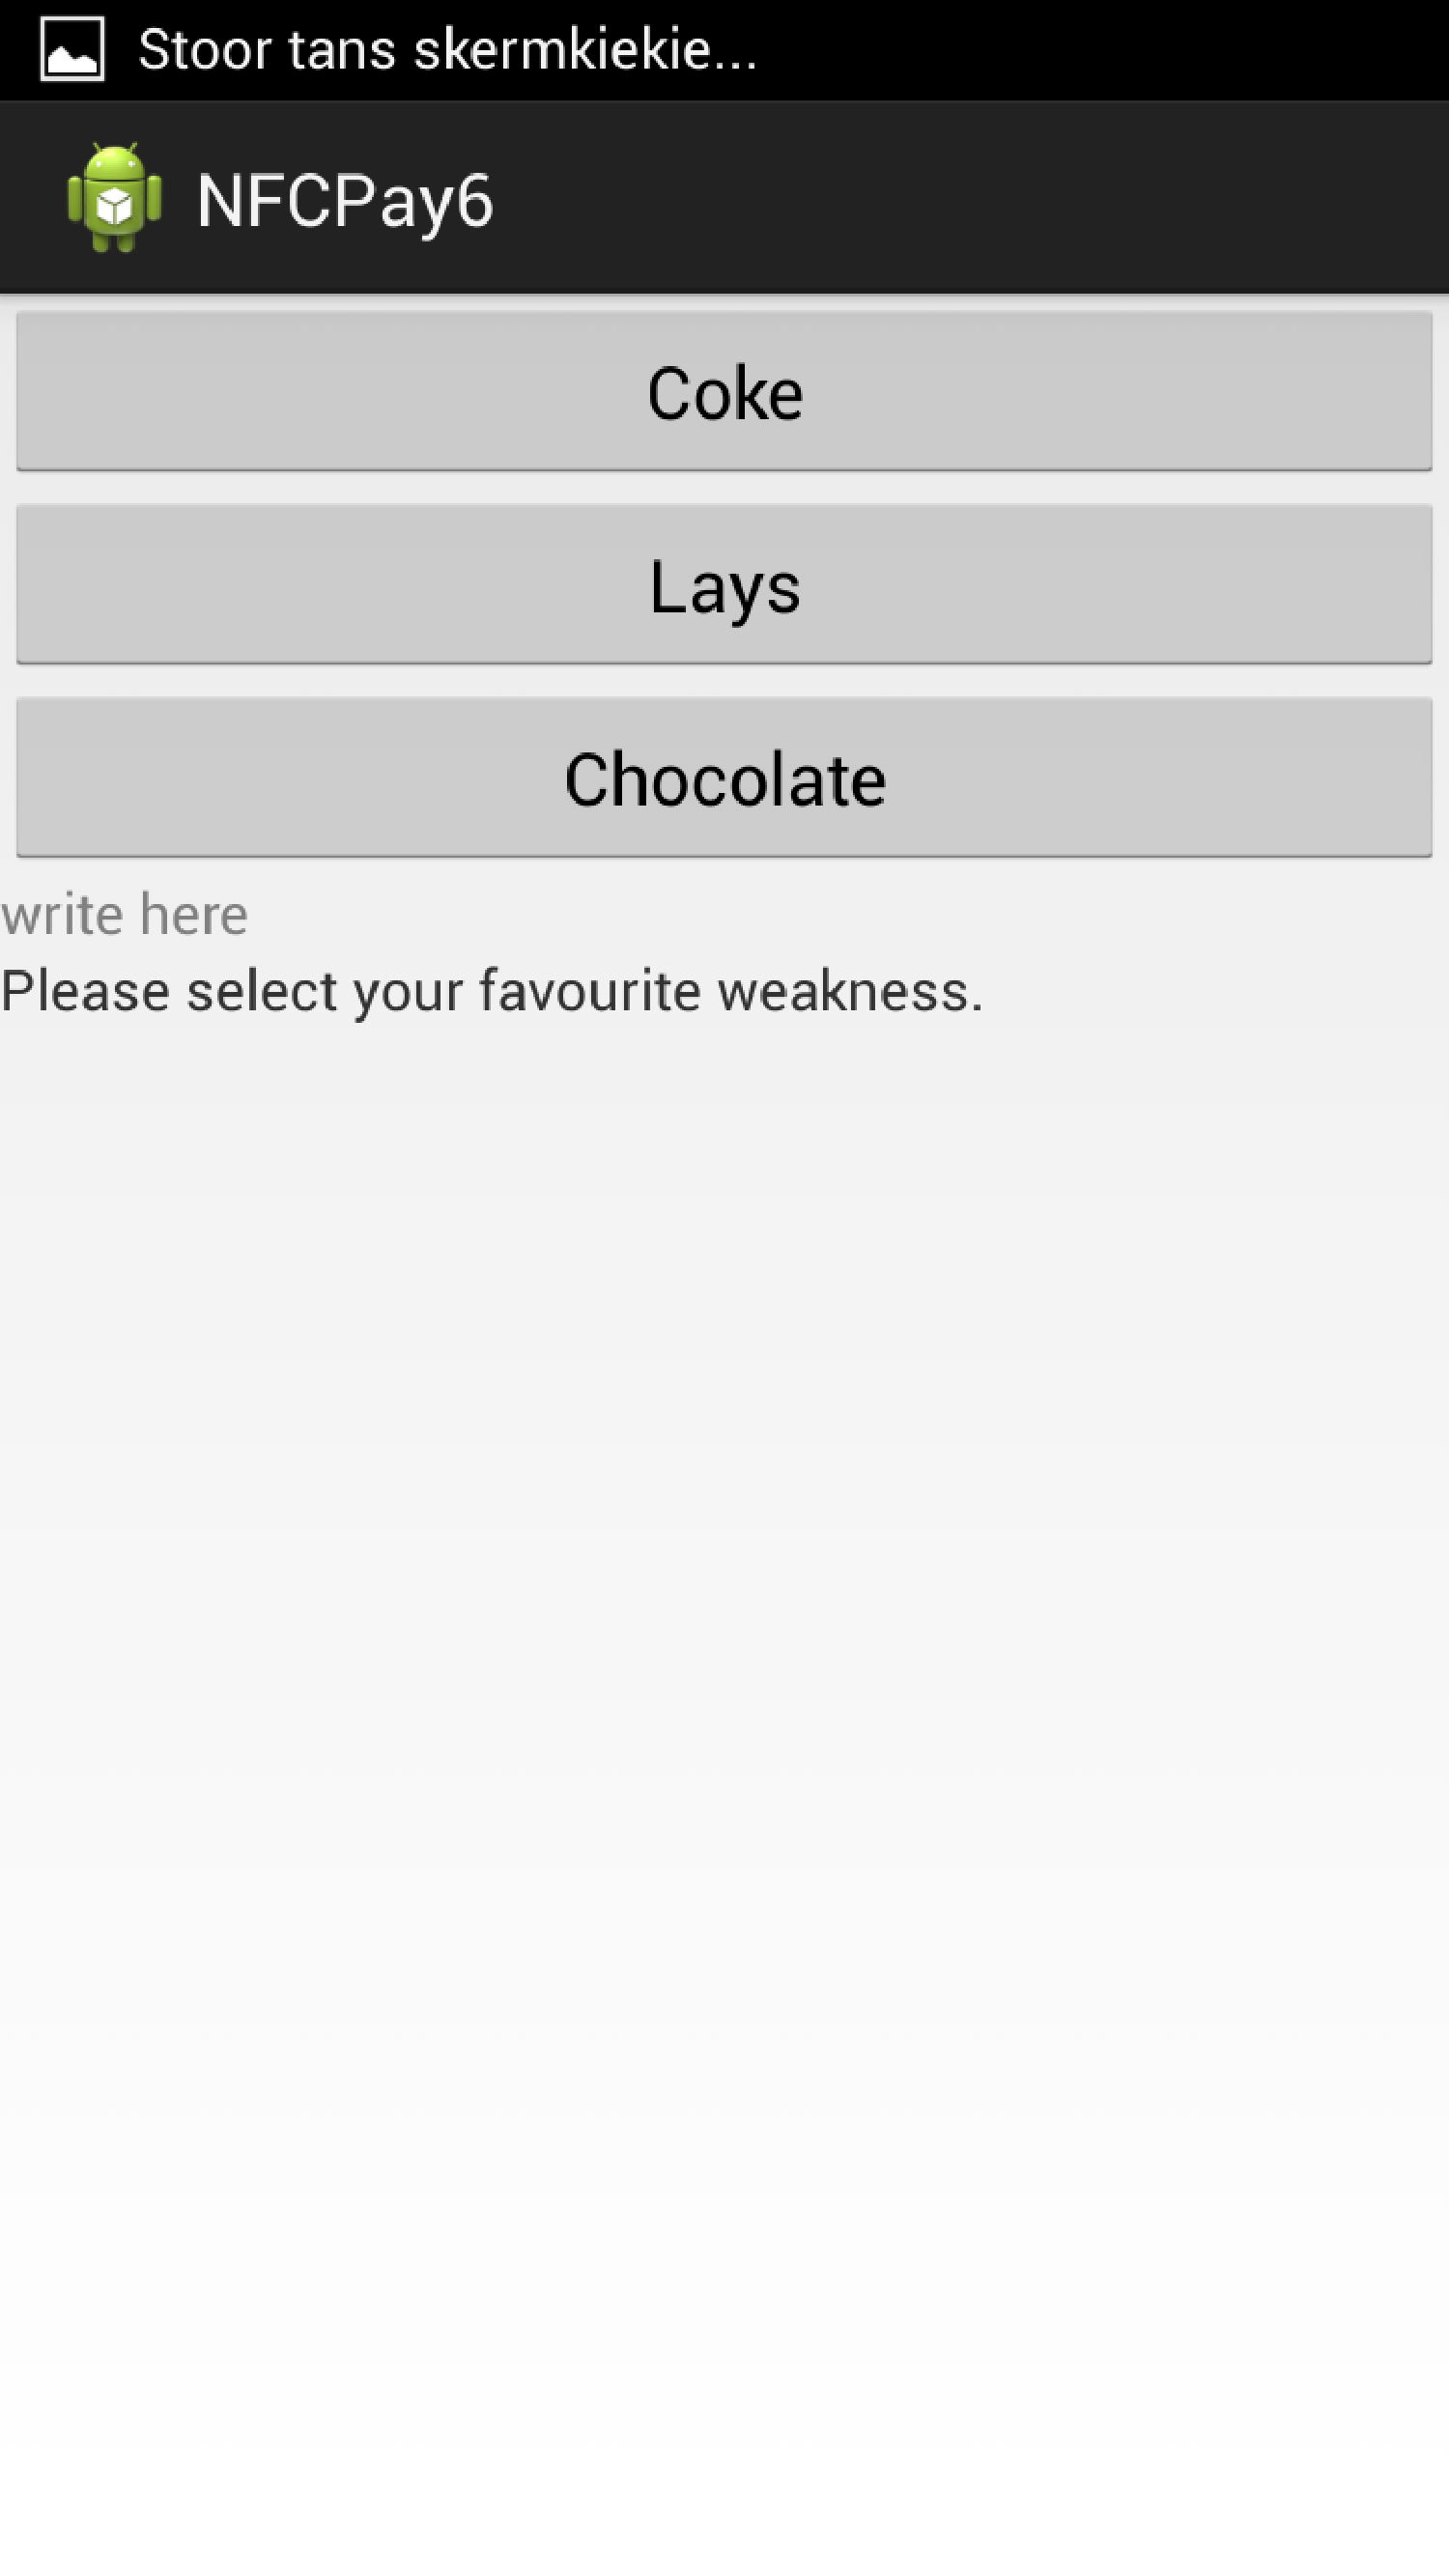
\includegraphics[clip = true, trim = 0 520 0 60,
 scale=0.2]{main_menu}
 \caption{A screenshot of the app's main activity activity}
 \label{fig:main-activity-screenshot}
\end{figure}

As seen from Figure \ref{fig:main-activity-screenshot}, the activity presents
the user with a list of products. When the user selects a product to buy, the
activity forms a data string by adding the product code, the user's login
name and password together. This data string is then encrypted with the
server's public key half and then encoded with base 64. This encoded string
is then embedded into a Uniform Resource Locator (URL) which points to the
web server. 

The activity then goes to this URL in the background which prompts the server to
process the transaction (see Section \ref{sec:app-nfc} for more details on the
server's NFC processes). The server then tells the activity if the transaction
has been approved or denied. If it has been denied, the user is informed what was wrong. 

If its approved, the activity activates the cell phone's NFC antennae which
transmits an encrypted approval message to the vending machine's NFC receiver. 

\chapter{System Tests}

\section{Transistor Switch}

\subsection{Current and Voltage Limits}

\subsection{}

\chapter{System Tests}

\section{Transistor Switch}

\subsection{Current and Voltage Limits}

\subsection{}

\section{User Tests}

\chapter{Conclusion}
\label{chap:7}

This chapter concludes this project design report. It gives a brief discussion on the
complete system and measures it against the project objectives set out in Section
\ref{sec:objectives} of this report. Lastly, it discusses possible improvements that can
be made to the system. 

\section{System Performance}

The project objectives set out in Section \ref{sec:objectives} of this report are repeated
here for convenience. They are:

\begin{itemize}
  \item The system must make provision for both NFC and Quick Response Code-based (QR
  Code) payments.
  \item The system must make use of a web server based in the cloud.
  \item An Android application must be made that will allow transactions to be completed
  using NFC.
  \item A demonstration model vending machine must be designed and constructed.
  \item All the data transfers between the user's cellphone and the server must be
  encrypted.
  \item Extra layers of security must be added. 
\end{itemize}

In the final system, both QR Code and NFC technology have been implemented. It was found
that the NFC option has a faster transaction time between product selection and
when the product is dispensed.
However, the NFC option is currently limited to cellphones that have NFC antennas and are
based on the Android Operating System.

It was found that the QR Code payment option typically has a slower transaction time. This
is mainly due to some hardware bottlenecks of the Pi. These bottlenecks include the
Raspberry Pi's moderate processing power, which increases the encryption time and the
time it takes the Pi to process and decode a live video stream from the webcam. These
bottlenecks may be improved with hardware modifications and processor overclocking. Extra
work can also go into optimising the code to make it run more efficiently. This can be
done by converting the code into compiled machine code.

Furthermore, a server has been made that runs in the cloud. This server interacts with a
customer's cellphone through the Android NFC application that was made or the cellphone's
internet browser. All data transactions between the server and the customer's cellphone
are encrypted with an asymmetric encryption scheme with extra layers of security added.

Lastly, a working demonstration vending machine was designed and made. It houses all of
the vending machine components and allows a customer to buy one of two products using
his cellphone. 

\section{Future Work}

The vending machine system that has been designed in this project has been designed to
work as planned. With that being said, there is potential to expand upon the work that has
been completed thus far.

This section discusses some potential improvements and additions that can be made to this
system

\subsection{Commercialisation}

The vending machine currently uses faux money which has no real-world value. Therefore,
the system in its current state is not ready to be deployed across Stellenbosch
University's campus. 

To commercialise the vending machine, third-party payment providers, such
as PayPal or PayPoint, can be integrated into the system. This will allow customers to
buy credits to use on the vending machine system by using their credit cards. 

All the transactions take place electronically and will therefore be integratable with the
current system. 

\subsection{Polish}

This project focused on the practical and functional aspects of the complete system and
almost no attention was given to the aesthetics of the complete system. Therefore, some
extra work can go into making the web server and Android NFC application more pleasant to use. 

\subsection{Integration}

One important aspect that must be focused on to increase the odds of making this project
more commercially successful, is its integration with current vending machines, i.e. add a
cashless option to current vending machines that are restricted to cash.

\subsection{More Payment Options}

Some work can go into expanding the number of payment options available to the user.

Some options that may be considered are Bluetooth, Instant Messaging (such as WhatsApp and
BlackBerry Messenger) and Unstructured Supplementary Service Data (USSD).


\appendix
%===========================================================

\chapter{Vending Machine Drawing}
\label{app:vm-tekeninge}
\chapter{Techno-Economic Report}
\label{app:techno-economic}

\section{Budget}

The planned total cost of completing this project was R532 000, with R12 000 going toward
manufacturing and components and R520 000 going toward the designer's salary.

The final cost for the design and manufacture of the complete system is R534 596. The cost
breakdown for this can be seen in Table \ref{tab:cost-breakdown}. The actual system value
is R14 596.

\begin{table}
\caption{Cost breakdown of the project and system}
\label{tab:cost-breakdown}
\centering
\begin{tabular}{|l|l|l|l|}
  \hline
  \textbf{Component} & \textbf{Amount required} & \textbf{Bought?} & \textbf{Cost when
  new} \\\hline\hline 
  12DC Motor & 2 & No & R4000 \\\hline
  NFC Controller & 1 & Yes & R780 \\\hline
  PS2 Eye Toy Webcam & 1 & No & R200 \\\hline
  12V Relay & 2 & No & R20 \\\hline
  2N2222 BJT & 2 & No & R5 \\\hline
  Vending machine unit & 1 & Yes & R107 \\\hline
  Raspberry Pi & 1 & No & R400 \\\hline
  HDMI Monitor & 1 & No & R5000 \\\hline
  Coils & 2 & No & R30 \\\hline
  Web server & 1 & No & Free \\\hline
\end{tabular}
\end{table}

Not all of the components used in this project were bought new. Some were loaned from
Stellenbosch University or elsewhere. Therefore, the actual cost of completing the project
is R520 887. 

Possible areas where saving can be made is to use smaller, cheaper motors and a smaller,
less expensive computer monitor. A smaller monitor will cost approximately R1000 and if
the system is integrated with a cash-based vending machine, the cost for the DC motors
will disappear. This gives a total system cost of R 3 596.

\section{Time Management}

This project was planned to be completed within 10 months. It was completed ahead of
schedule. A Gannt chart showing the project timeline can be seen in Figure \ref{fig:gannt}
in Appendix \ref{app:c}.

\section{Technical Impact}

This project produced a vending machine which accepts payments made via cell phone.
Allowing customers to pay using only their cell phones makes an already convinient service
even more convenient. 

The prototype system was designed with expansion and modification in mind an is not
necessarily restricted to vending machines.
For example, the system will accept any cell phone payment made at any vendor if it is
properly modified and configured. 

\section{Return on Investment}

\textbf{[Prof. van Rooyen: Dit voel vir my die potential for commercialisation is klaar in
hierdie afdeling behandel. Moet ek dit opbreek in twee dele liewers, of kan ek dit so
hou?]}

As discussed in Section \ref{sec:final-system-goal} of the main report, cashless
transactions are expected to surpass cash transactions by the year 2015. It is therefore
very important for vendors to keep up with the trend and allow customers to pay with
cash, but still provide a cashless payment facility. 

This project has delivered a working cashless vending machine, but the system can be
expanded upon and adapted to be integrated with traditional, cash-based vending
machines. This integration will require more research and development, however, but it
will be worth it to give modern shoppers a choice between paying with or without cash.

To get to this point, an estimated R2.3million will be required. R1.1million will go
toward paying the developers' salaries, R1million toward setting up data servers and paying their
overhead costs, R100 000 for components and manufacturing costs and a final R100 000 for
buying at least three standard cash-based vending machines to test the final system. 

When the final system is complete, it presents a few opportunities for investors to make
money. Firstly, the systems can be manufactured by the development company and sold to
vending machine manufacturers. Second, it can be manufactured under license by the vending machine
manufacturers, with the development company receiving royalties. Lastly, the system can be
patented and the patent can be sold to another company for a premium. 

If the system is manufactured in-house, it will cost approximately R3 596 to make. If
these systems are then sold to vending machine manufacturers at R7000 per unit and 210
units are sold per year, the original investment will be remade approximately 4 years,
not accounting for inflation. This gives a return of 18.9\% per year.

If these systems are manufactured under license by vending machine companies, and
royalties are received in the amount of R2300 per unit made with 210 units made per year,
it will take 6 years for the investors to remake their money. This gives a rate of return
of 12.2\% per year. 

Lastly, if the patent is sold, it will have to be sold for at least R2.9million to make up
for the initial investment. It is highly unlikely that a company will spend this amount of
capital on an unproven system. If it is sold for R3million, it will immediately give
investors a return on their investment. However, the long-term revenue generated by the
other two options far outweigh this R3million and it is therefore recommended that the
first two options be considered.

\chapter{Updated Gannt Chart}
\label{app:c}

\begin{figure}
 \centering 
 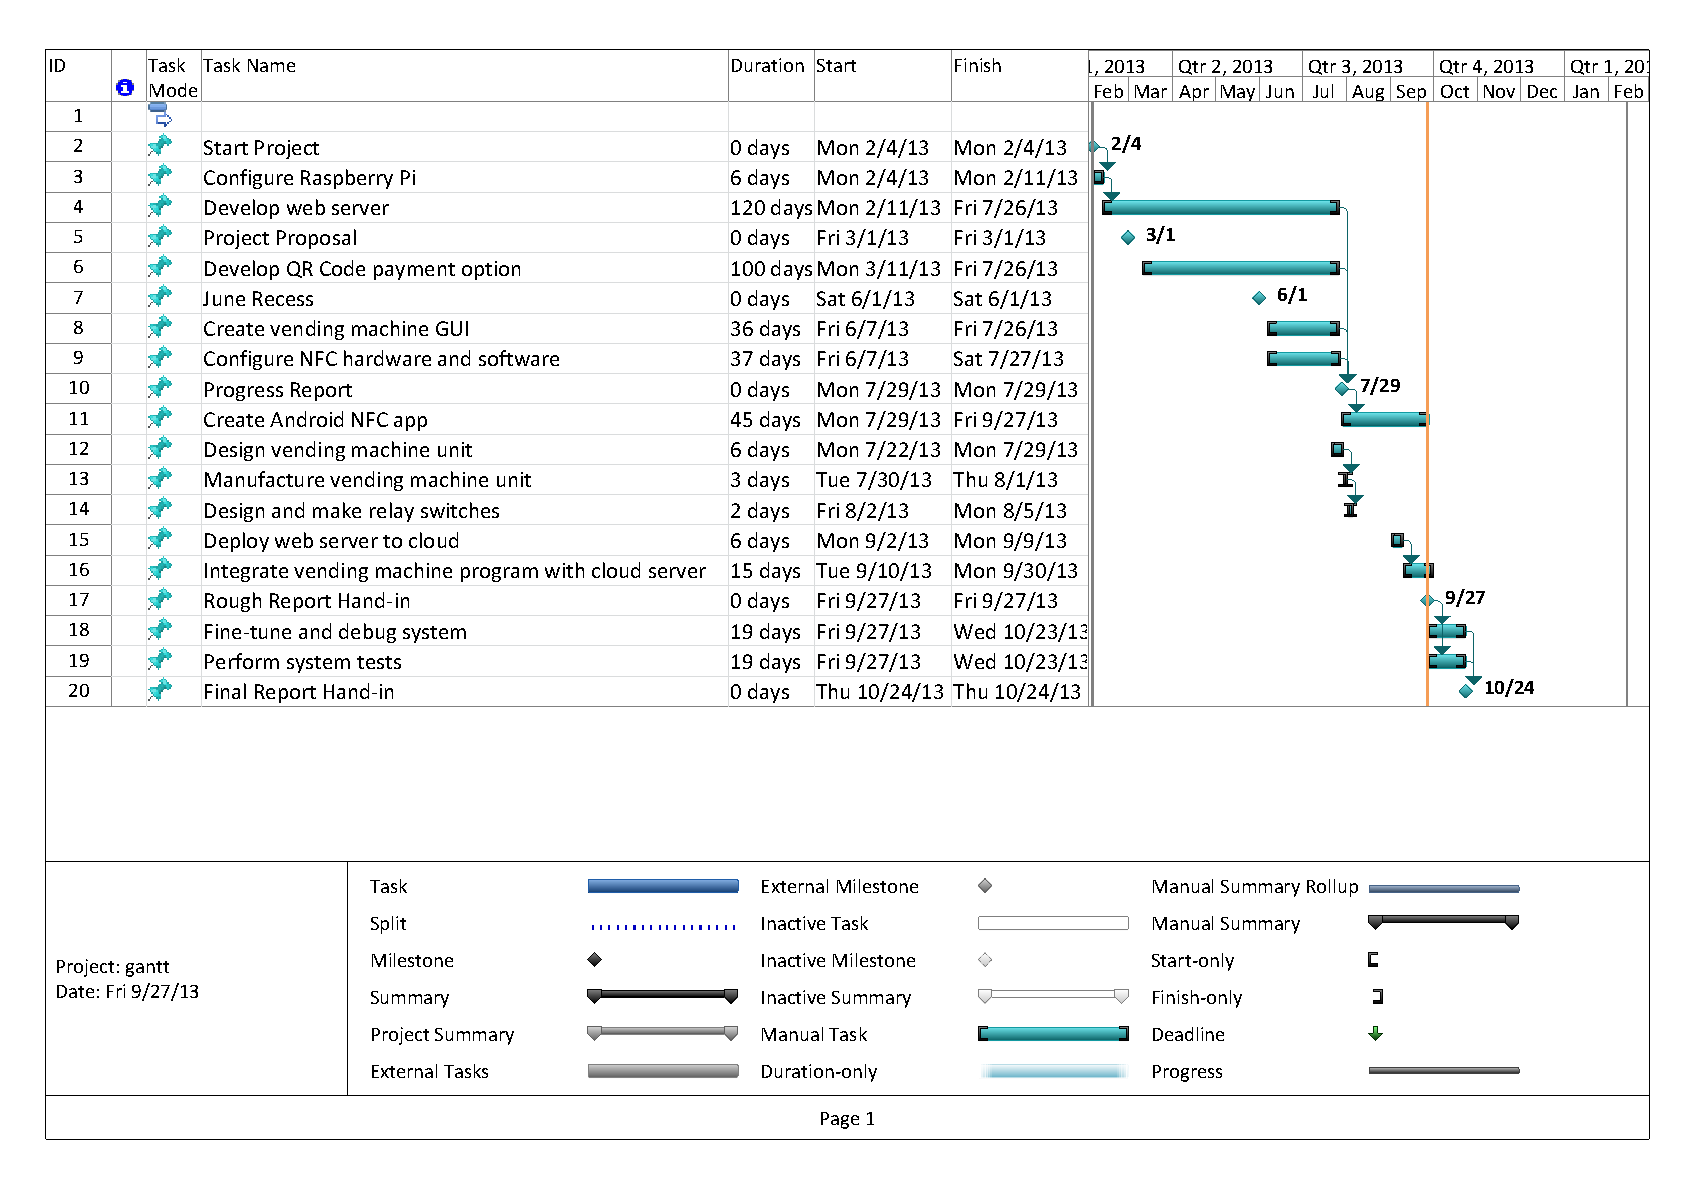
\includegraphics[clip=true, trim = 0 0 0 0,
 scale=0.68, angle=270]{gantt}
 \caption{Gannt Chart showing the project timeline}
 \label{fig:gannt}
\end{figure}
\chapter{System Hardware Schematic}
\label{app:d}

\begin{figure}
 \centering 
 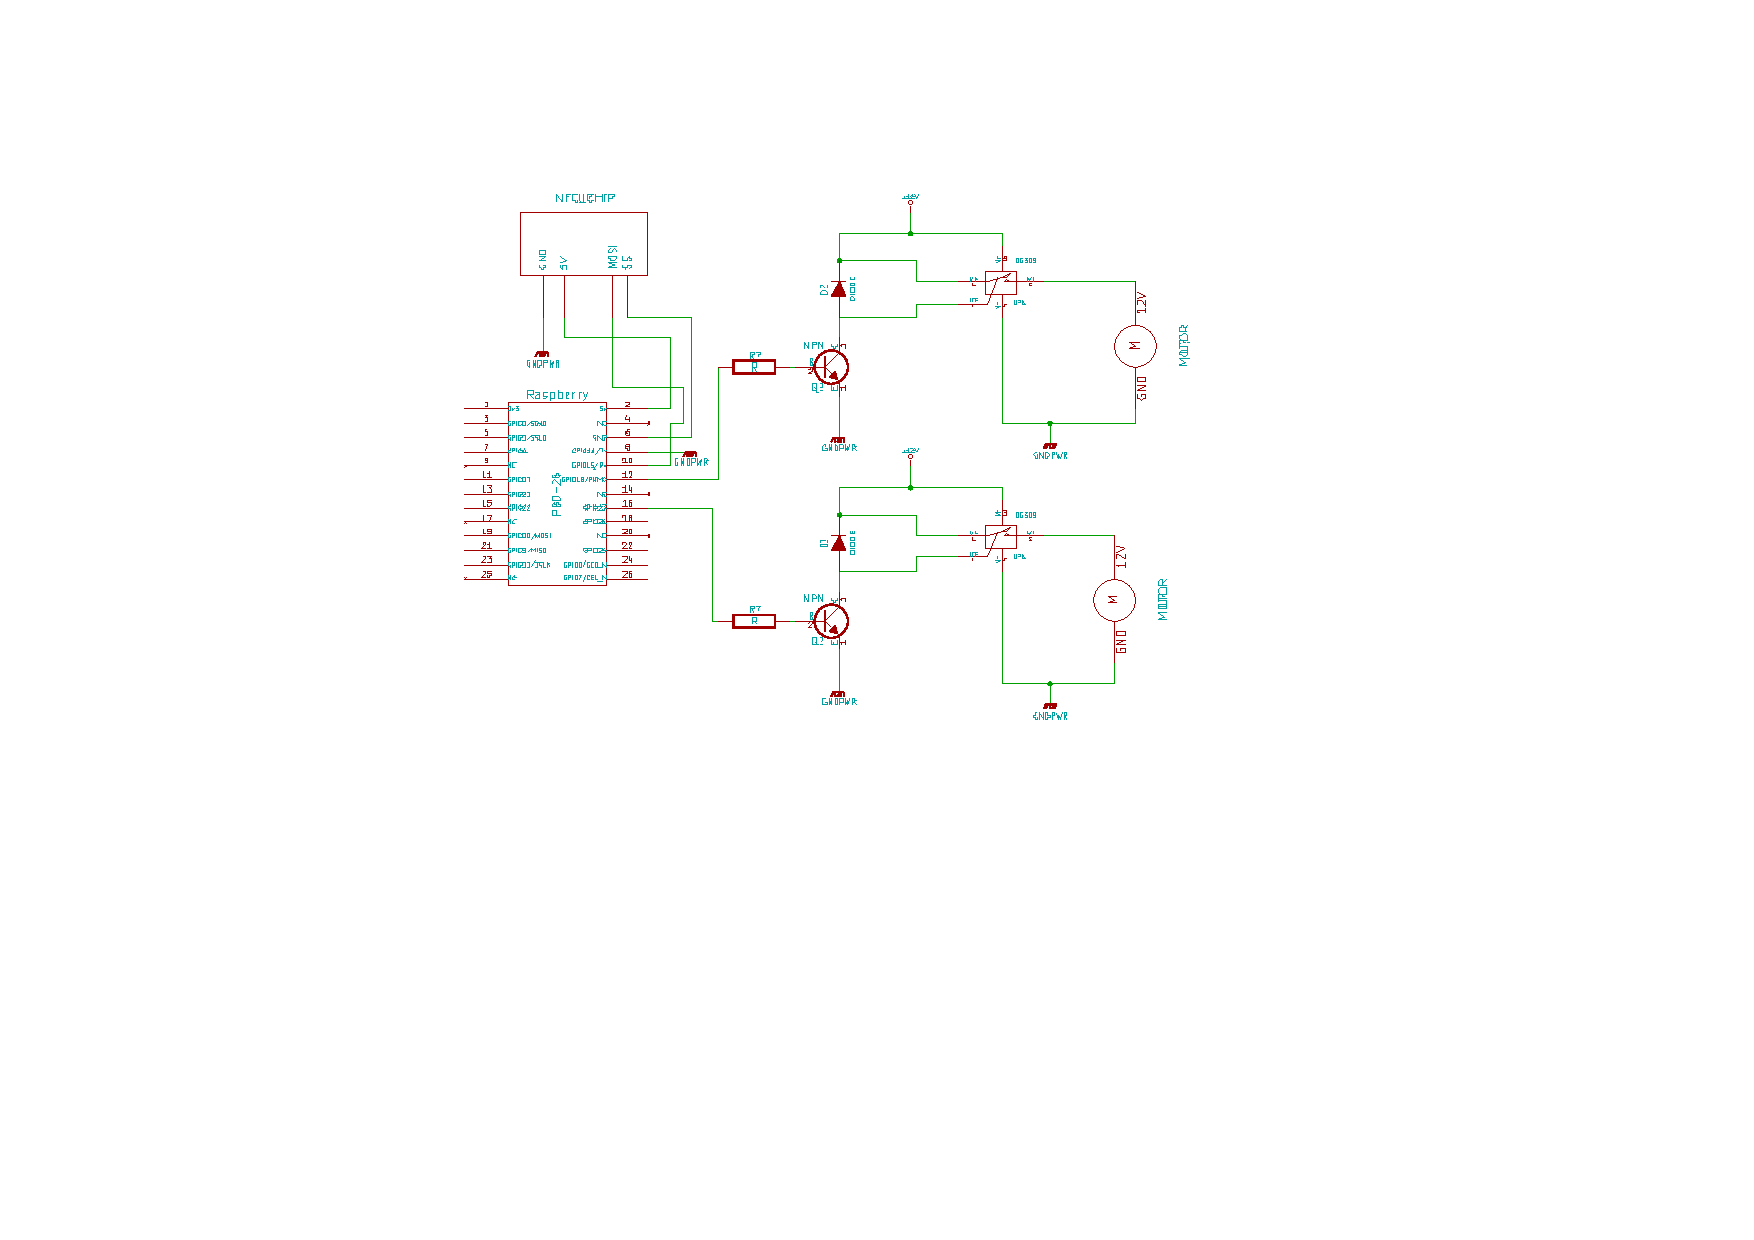
\includegraphics[clip=true, trim = 230 250 0 90,
 scale=1.4]{system_schem}
 \caption{Schematic of the complete system.}
 \label{fig:hardware_schem}
\end{figure}
\chapter{Asymmetric Encryption}
\label{app:ass-encryption}

Asymmetric encryption is most easily explained with a postal analogy:

Imagine that two people, Alice and Bob, want to send each other secret messages through
the public mail. In other words, Alice wants to send Bob a secret message and she expects
a secret reply from Bob, and vice versa. 

In an asymmetric scheme, Bob can lock his letter to Alice with a padlock to which only she has
a key (she keeps this on her person at all times and does not show it to anyone, which
includes Bob). This open padlock represents the public key half of Alice's key. This
means that anyone can send Alice a secure message with a public key, which is easy to
get from Alice, and only Alice can unlock the message with her private key half of the
key pair. Similarly, Alice can lock her letter with Bob's padlock which only Bob can open.

The great advantage that this has over symmetric encryption is that the decryption keys never
have to be exchanged between parties. This neutralises the risk of a middle-man attack,
analogous to a nosy postal worker called Eve who likes to read other people's
mail, who then intercepts the message and steals the key. Also, if for example Bob has
been careless and allowed Eve to see his key, his messages to Alice will be
compromised. However, the messages from anyone else (including Bob) to Alice
will remain as secure as it was before Bob lost his key.

The data source can also be signed and verified by using this key scheme. Referring once again
to the postal analogy: To show Alice that it was indeed Bob who sent her the
message, and not Eve for example, he can send an extra message along with the
original message. This extra message is locked with Bob's key that he shares
with no one (i.e. his private key). However, Bob has sent out his public key to
everyone who wants it. These keys can \emph{only} be used to unlock the
messages locked with Bob's own private key. Therefore, if Alice, who received
one of Bob's keys, can unlock this extra message with that key, she knows that
as long as Bob has not given anyone his private key, it can only be his
message. The reverse is also true if Alice wants to prove to Bob that it was
indeed she who sent him a message.
\chapter{Server Configuration}
\label{app:server-config}

\section{Elastic Compute Cloud}

The AWS EC2 server provides the platform on which the Apache
server runs. The EC2 server instance was configured to run
Ubuntu 12.10, `Quantal Quetzal'. This was done because most
of the server development was done on Ubuntu 12.10, and the
server code will therefore require minimal adaptation to be able to run on the EC2
server.

After the server instance was created, the following
packages and programs were installed for the server to be able to run properly:

\begin{itemize}
  \item Apache2: Installs the Apache server framework.
  \item libapache2-mod-wsgi: An Apache module that allows Apache to work with
  Python Web Server Gateway Interface (WSGI) scripts.
  \item python-pip: Allows Ubuntu to install Django from the Python Package Index (PyPI)
  [\cite{website:pypi}].
  \item Django: Installs the all the Django packages that will be used by the server. 
\end{itemize}

Because the server's database uses SQLite3, which is part of the standard Ubuntu
12.10 distribution, no external database programs were needed to be installed.

After this was completed, the server is fully capable of serving Django web
pages.

\section{Apache Configuration}

The Apache server framework provides the foundation on which the Django server runs. It had to
be configured to be able to run the Python scripts that Django contains. To do this, the steps
described in Nick Polet's blog post was followed [\cite{article:apache-setup}]. It describes
in detail how to configure Apache to serve a Django website.

For Apache to be able to serve Django sites, it had to be configured to run the Web Server
Gateway Interface (wsgi.py) script located within the Django server folder. This was done by
adding the following code to the Apache's httpd.conf configuration file:

\begin{verbatim}
WSGIScriptAlias / /home/ubuntu/srv/server_site/server_site/wsgi.py
WSGIPythonPath /home/ubuntu/srv/server_site

<Directory /home/ubuntu/srv/server_site/server_site>
<Files wsgi.py>
Order deny,allow
Allow from all
</Files>
</Directory>
\end{verbatim}

The following line was also needed to be added to Apache's apache2.conf file:

\begin{verbatim}
Include httpd.conf
\end{verbatim}
\chapter{NFC Chip Configuration and libnfc Setup}
\label{app:nfc-chip-config}

To make the Raspberry Pi serially communicate with the NF Chip, the `SEL1'
pads were shorted (see Fig.
\ref{fig:nfc-chip-solder}). With this done, the chip can serially communicate
with the Raspberry Pi's UART interface.

\begin{figure}
 \centering 
 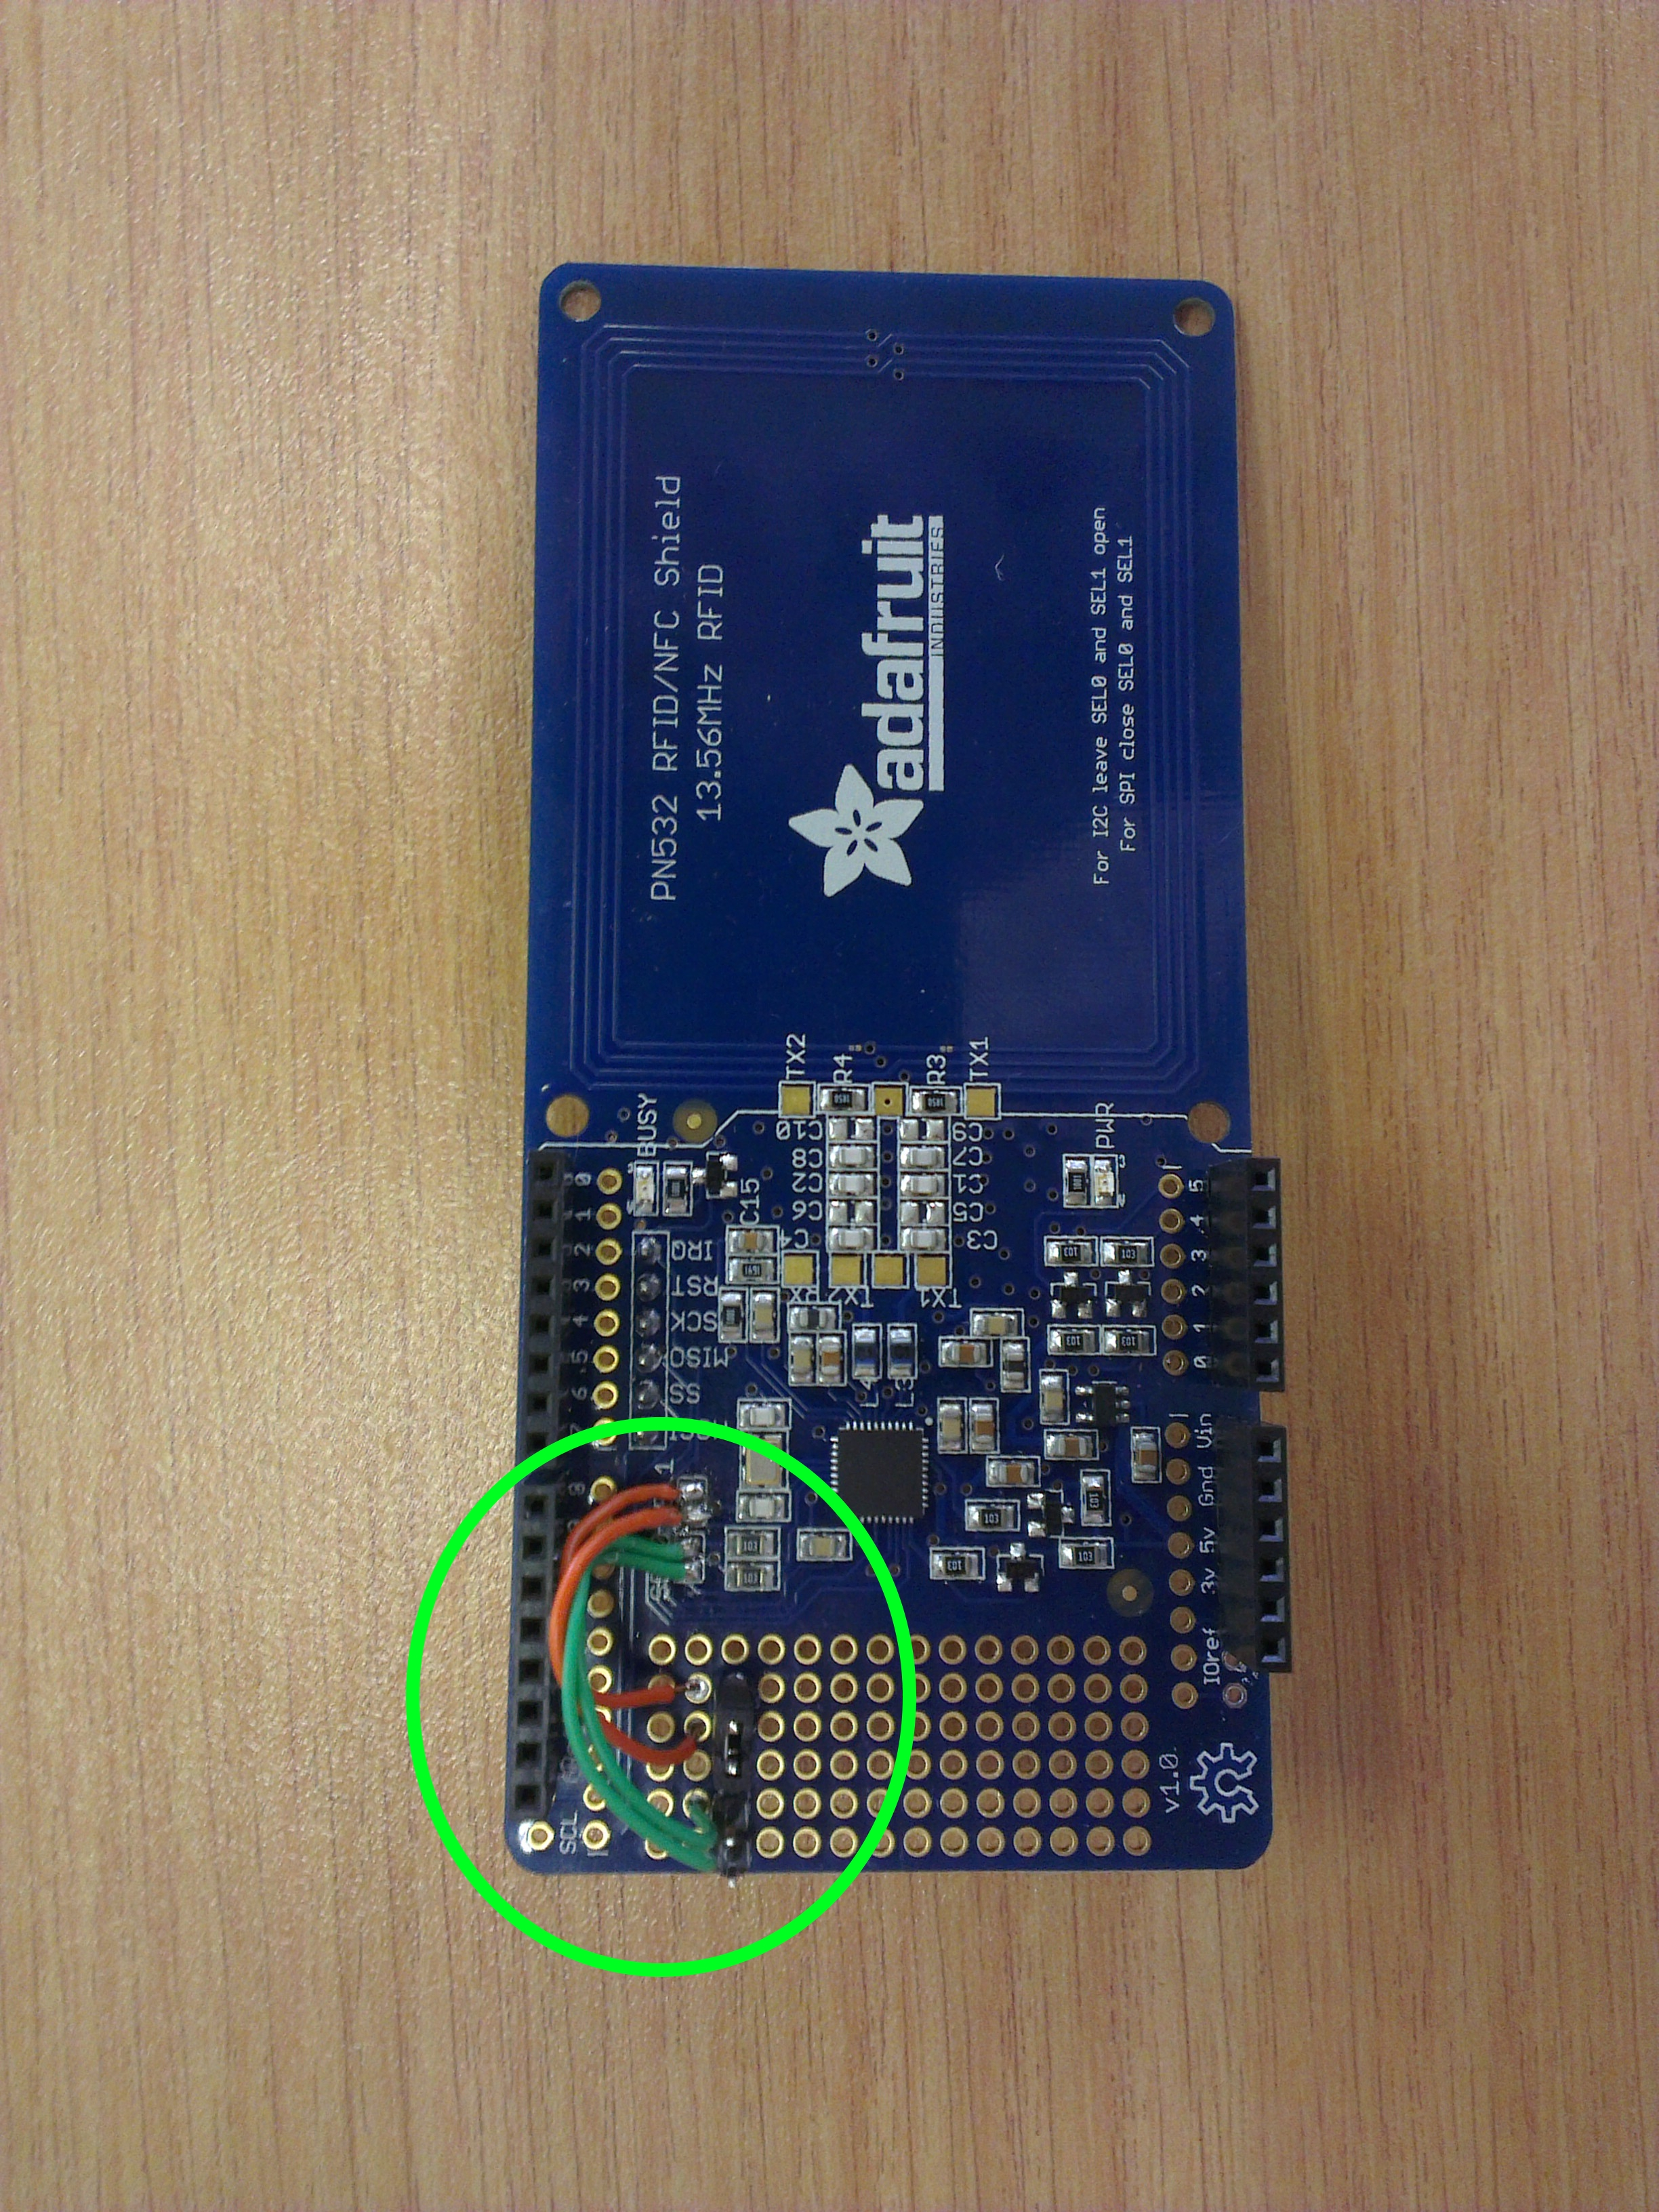
\includegraphics[clip=true, trim = 0 250 0 290,
 scale=0.7]{soldeer_pic}
 \caption[The location of the SEL1 pads.]{The location of the SEL1 pads (highlighted in
 green).}
 \label{fig:nfc-chip-solder}
\end{figure}

The connections between the Pi and the NFC controller are given in Table
\ref{tab:chip-connections}.

\begin{table}
\centering
 \caption{Connections between the Raspberry Pi and the NFC Controller chip.}
 \begin{tabular}{|l|l|l|}
  \hline
  \textbf{NCF Controller Pin} & \textbf{Raspberry Pi Pin}\\\hline\hline
  5V pin & 5V (pin 4) \\\hline
  Ground pin & Ground pin (pin 6) \\\hline
  SS & UART0 TXD (pin 8) \\\hline
  MOSI & UART0 RXD (pin 10) \\\hline
 \end{tabular}
 \label{tab:chip-connections}
\end{table}

\section{libnfc Setup on the Raspberry Pi}

Before libnfc could be built and configured, a communication line between the NFC
controller and the Pi needed to be opened. To do this, the Pi's UART needed
to be freed up. By default, the Raspberry Pi uses its UART to serially write out
its booting information. Therefore, to allow the Raspberry Pi to communicate
with the NFC controller via its UART0 interface, it was necessary to modify
some of its configuration files. To do this, the Adafruit tutorial was followed
[\cite{website:adafruit-tutorial}].

The file `/boot/cmdline.txt' and `/etc/inittab' had to be edited to
contain the following lines of code:

\textbf{cmdline.txt}
\begin{verbatim}
dwc_otg.lpm_enable=0 console=tty1
\end{verbatim}

\textbf{inittab}
\begin{verbatim}
#Spawn a getty on Raspberry Pi serial line
#T0:23:respawn:/sbin/getty -L ttyAMA0 115200 vt100
\end{verbatim}

After this was done, the libnfc package could be configured and installed 
to work with the Pi's UART interface.

Thereafter, the Pi was ready to receive NFC messages from the NFC shield.
\chapter{ECSA Outcomes Self Evaluation}
% Table generated by Excel2LaTeX from sheet 'Sheet1'
\begin{longtable}{|p{5.9cm}|p{2.2cm}|p{5.5cm}|}
\hline
{\bf Outcome} & {\bf Location} & {\bf Description} \\
\hline
{\bf 1.  Problem Solving} &            &            \\
1.1 Problem  identification & Section 1.1 & The problem is formulated and
explained here. \\

1.2 Set solution criteria & \parbox[t]{5cm}{Section 1.3 \\
Section 1.4} & The project goal and system objectives are explained here. \\

1.3 Identify solutions & \parbox[t]{5cm}{Section 1.2 \\
Chapter 2} & Existing solutions, such as USSD and NFC are discussed here. \\

1.4 Solve problem & \parbox[t]{5cm}{Chapter 4 \\
Chapter 5} & The system design is discussed in these chapters. \\
\hline
{\bf 2. Application of scientific engineering knowledge} &            &            \\
2.1 Use fundemental physics used to solve problems & Section 5.1
Section 5.5 & Basic electro-technicques and mathmatical laws are used here to design a relay switch circuit and a vending machine coil. \\

2.2 Integrate different systems &            & This project required a physical system (the vending machine unit and its hardware) to be integrated with software systems (the server and the vending machine control program). This required careful planning and execution of the plan. \\
\hline
2.3 Electronic design & Section 5.1 
Section 5.2 & Used fundamental electric and electronic design principles to
identify circuit requirements, choose components and build the circuit. \\
\hline
{\bf 3. Engineering Design} &            &            \\
3.1 Acquire background knowledge &  Chapter 2 & This chapter gives the background information on all the tools and concepts that were required to design a successful system. \\

3.2 Generate concepts & Section 1.2 & Here different payment options are listed.  \\

3.3 System design &  Chapter 3 & This chapter discusses the complete system design. Project design choices are made and motivated here and unfamiliar concepts are explained.   \\

3.4 Detail Design & Chapter 4
Chapter 5 & These chapters discuss the detail design of the software and hardware components of the project. This includes mathematical motivations for the  design choices made.  All hardware and software configuration is also discussed. \\

3.5 Design evaluation &  Chapter 6 & This chapter discusses the perfomance of the completed system. Evaluations of each of the payment methods are made and discussed. User tests are also performed and discussed. \\

3.6 Plan and manage project & Appendix C & Here a Gannt chart is given of the project planning. This plan was followed throughout this report. \\
\hline
3.7 Assess impacts of the design & Appendix B & Here is a socio-economic report that discusses the potential economic impact that this system may have.  \\

3.8 Use CAD as design tool & Section 5.3
Appendix A & Designed and manufactured a working vending machine unit using CAD software \\
\hline
{\bf 4. Investigations, experiments and data analysis} &            &            \\
4.1 Plan and conduct tests &  Chapter 6 &            \\

4.2 Select software & Section 6.1 & The Dstat load monitoring software was identified, tested and selected for system tests. \\

4.3 Analyse data & Sections 6.1 - 6.10 & For every test conducted, the data was analysed using MS Excel and presented on a reader-friendly graph.   \\

4.4 Draw conclusions based on data &  Chapter 6 & A conclusion to each test was given and motivated. \\

4.5 Communicate purpose, process and outcomes &  Chapter 6 & The purose of each test, the steps taken during the tests and the results of each test was discussed and motivated in this chapter.  \\
\hline
{\bf 5. Engineering methods, skills and tools, including IT} &            &            \\
5.1 Select appropriate programming language & Section 4.1
Section 4.2 & Python was selected to create a web server, the vending machine's GUI and to control the vending machine. \\

5.2 Successfully create computer and cellphone applications and programs &  Chapter 4 & This chapter discusses a web server, a vending machine program and an Android app thatw as created for this project.  \\

5.3 Correctly configure and use hardware & Section 5.2
Section 5.4 & The NFC Chip and webcam had to be configured to be compatible with the Raspberry Pi.  \\
\hline
5.4 Successfully design system using engineering design principles &            &            \\

5.5 Display knowledge of manufacturing methodologies and constraints & Appendix A & A manufacturable vending machine shell was designed and manufactured. Bending and, laser-cutting and welding were used in this process. \\

5.6 Display competency in processing data &  Chapter 6 & MS Excel software was used to process the test data and display the results on a graph.  \\
\hline
{\bf 6. Proffesional and technical communication} &            &            \\
6.1 Witten communication & This report
Previous reports & Graphs and tables are used where appropriate. Correct language used thoughout the report. Acronyms and terms are properly defined and consistently used. Referencing to outside sources are also used throughout the report.  \\

6.2 Oral communication &            & Not applicable in this report. \\
\hline

{\bf 8. Individual, team and multi-disciplicary working} & &\\

8.1 Moderate supervision required & Main report preamble & Supervisor, Prof. G-J
van Rooyen credited in Ackknowledgements section of the main report. \\

8.2 Project completed within deadline & & Project handed in before deadline \\

8.3 Objectives met and project well-planned & Chapter 1 and 7
Appendix C & Here the project objectives are set and it is discussed if the
project has met them. A Gannt chart is alsoe given showing the project planning.
\\\hline\newpage\hline

{\bf 9. Independent learning ability} &            &            \\
9.1 Learn new programming langues &            & Skills in using Python and Java were required and acquired in this project. Android, Django and EC2 also required some familiarisation and learning.  \\

9.2 Familiarise self with new Operating Systems. &       Chapter 3     & This
project required that one be able to work on Linux-based computers. It also required basix knowledge on how Android applications work. \\

9.3 Familiarise self with new hardware and sensors. &      Chapter 3      &
Knowledge on how a Raspberry Pi and the NFC protocols work was required.  \\

9.4 Learn new concepts &       Chapter 2
Appendix E     & An understanding of how
public key encryption works was required. Additional security measures also had  to be studied and implemented. \\

9.5 Critically evaluate self & \parbox[t]{5cm}{Section 6.10\\
Chapter 7} & Faults were found in the finished system and recommendations were given on
how they could be fixed. Future work and improvements that can be made are also given and discussed.  \\
\hline
\end{longtable}  

\backmatter
%=========================================================

\raggedright
\footnotesize
\bibliography{bibliography}

\end{document}